\documentclass[a4paper, twoside]{article}
\usepackage[fontsize=10pt]{scrextend}
%\documentclass[10pt]{extarticle}
\usepackage[T1]{fontenc}
\usepackage[utf8]{inputenc}

\usepackage[margin=1in]{geometry}
\usepackage{amsfonts, amsmath, amssymb}
\usepackage{mathtools}

\usepackage{graphicx}
\usepackage{subfig}

\usepackage{url}
%%  Defines the command \url{} that can be used to typeset url:s
%%  in text

\usepackage[parfill]{parskip}
\usepackage{ragged2e}

\setcounter{tocdepth}{4}
\setcounter{secnumdepth}{4}


\newcommand*{\pd}[2]{\ensuremath{\dfrac{\partial #1}{\partial #2}}}
\newcommand*{\inpd}[2]{\ensuremath{\frac{\partial #1}{\partial #2}}}
\DeclarePairedDelimiter\floor{\lfloor}{\rfloor}

\title{Derivation of a Convolutional Neural Network Based Dense Face Detector}
\title{Dense Face Detection with Convolutional Neural Networks}
\author{Nikita Zozoulenko \\*
nikita.zozoulenko@gmail.com \\*
Katedralskolan Linköping\\*
Supervisor: Rickard Engström \\*}

\begin{document}
\maketitle

\vfill
\begin{figure}[h]
	\centering
  		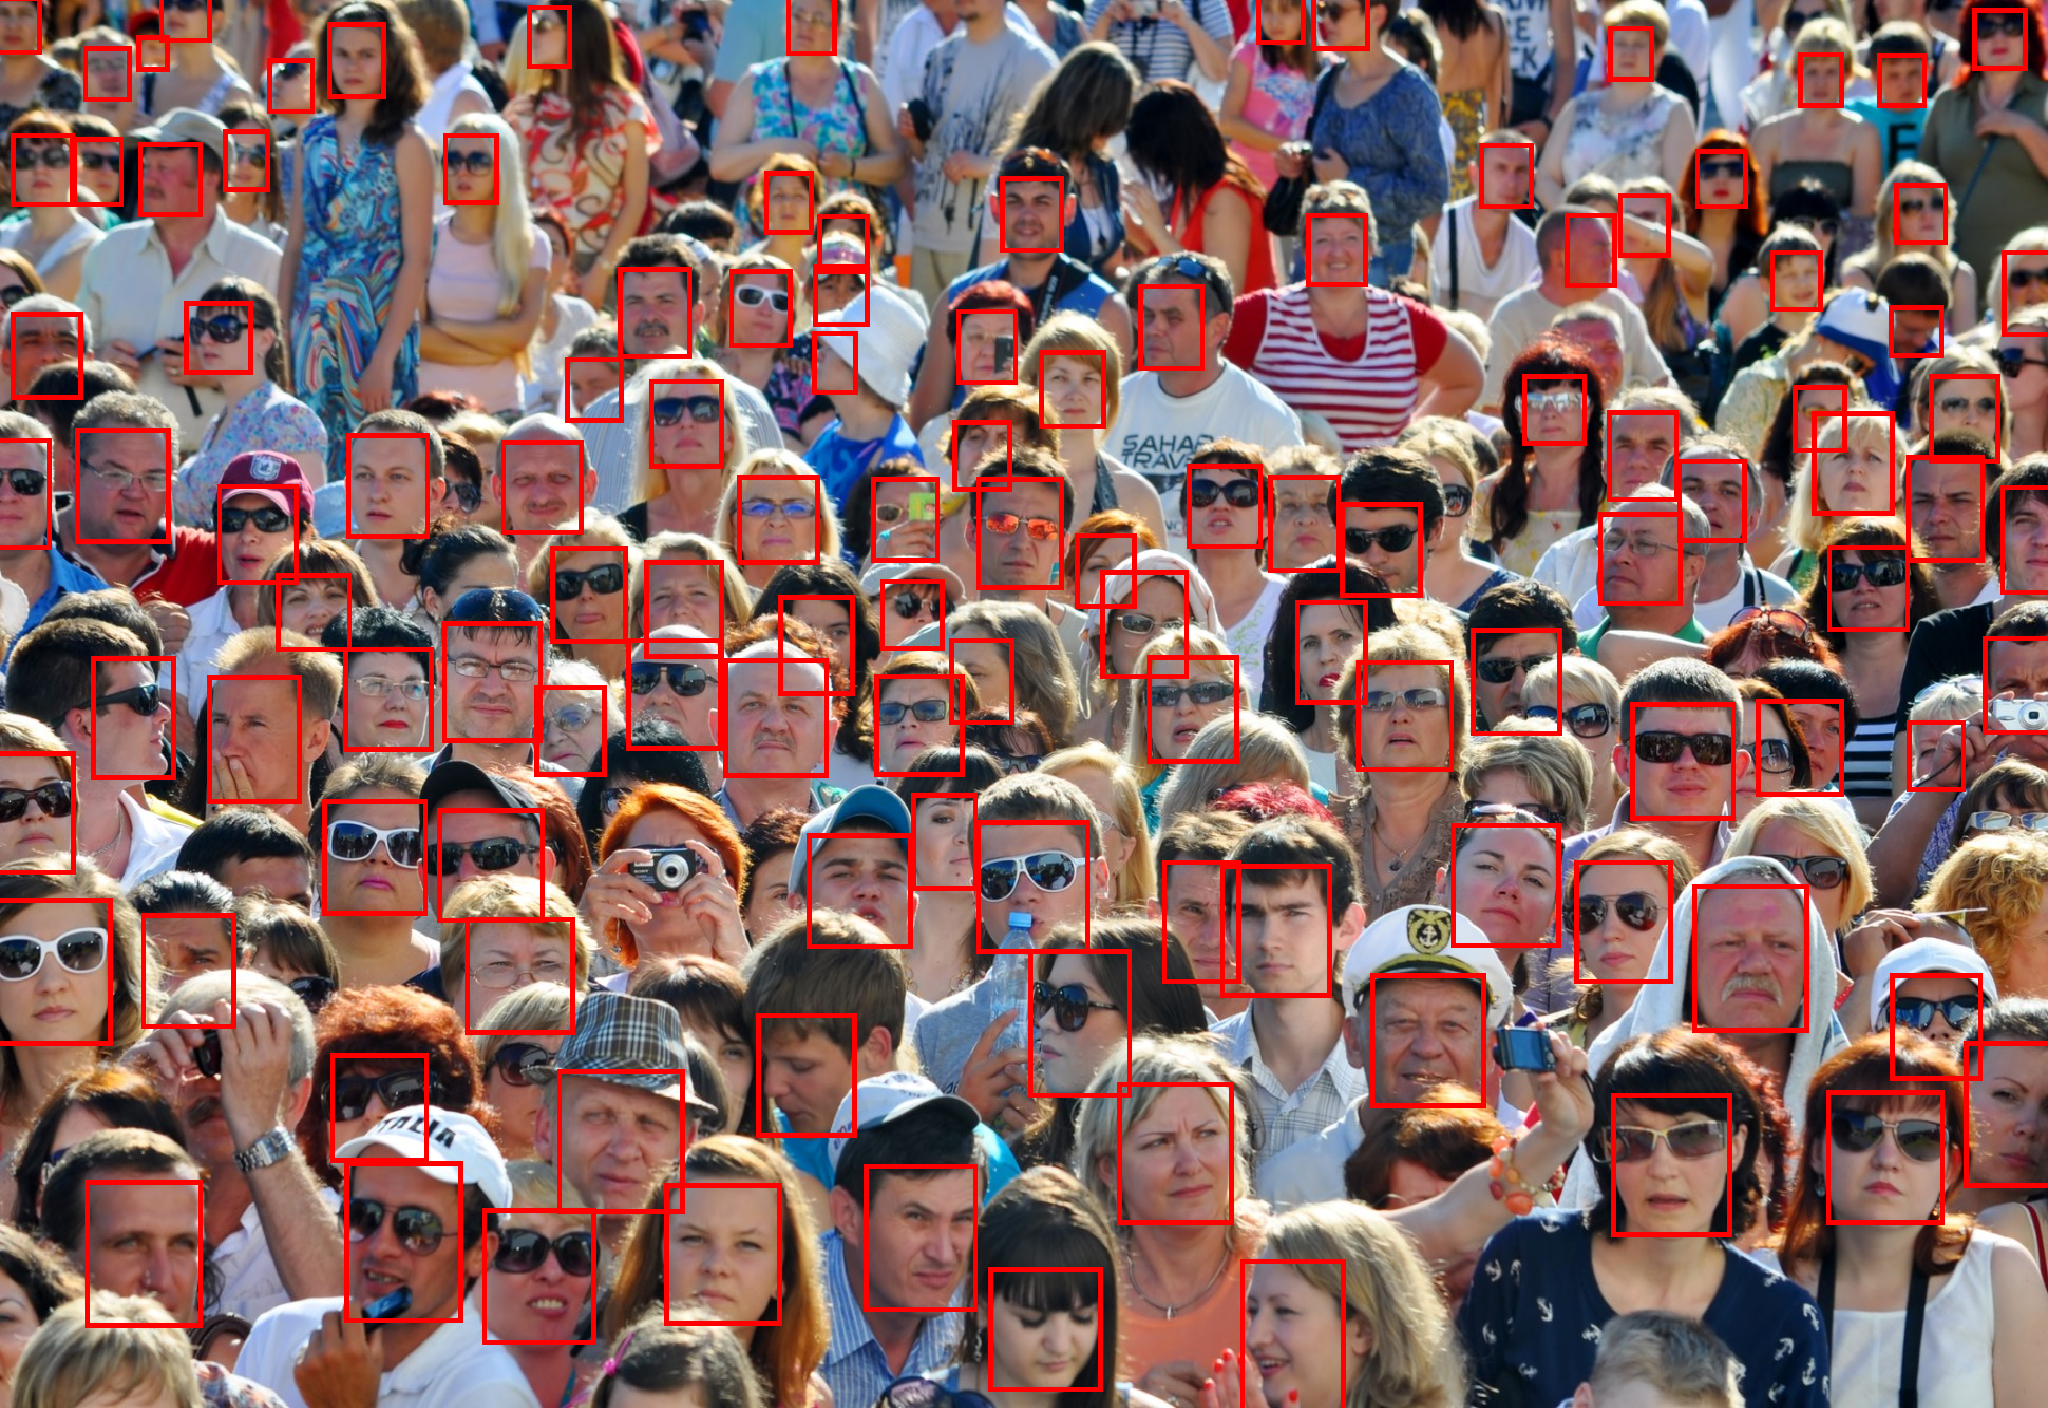
\includegraphics[scale=0.221]{resultscrowd2.png}
  	\caption{The proposed convolutional neural-network-based model FaceResNet is capable of dynamically detecting over 200 faces in a crowded scene for various scales, lighting and occlusions. A detection is shown as a red boudning box.} \label{crowd}
\end{figure}
\vfill

\newpage

%start abstract
\Large{\textbf{Abstract}}\\

Convolutional neural networks are currently the state of the art model for tasks such as image classification, image recognition and object detection for computer vision systems. In this paper the mathematical model behind the standard feed-forward neural network and the convolutional neural network is derived. The performance of two models, a convolutional neural network and a feed-forward neural network, are then compared on the task of classifying handwritten digits. A convolutional neural-network-based model is then constructed to make a cutting edge face detector for real time video, being able to successfully detect over 200 faces in a crowded scene for various scales, lighting and occlusions.
\newpage
%end abstract

\tableofcontents
\newpage
\section{Introduction}

\subsection{Background}

An Artificial neural network is a biologically inspired machine learning model that tries to replicate the way the brain in mammals functions. There are many different kinds of Artificial neural networks which vary in structure and architecture. The basic principle behind neural networks is that they are made up of a number of layers of neurons. The layers are built sequentially such that the output of one layer is the input to the next layer. The number of layers a neural network is constructed out of is called its depth. How the neurons of the previous layer are connected to the neurons of the next layer depends on the specific type of artificial neural network \cite{cs231n}.

Similar to other machine learning models, an artificial neural network wants to predict a predetermined number of values, given an input of a number of data points. For instance, a neural network can be given $784$ pixel values from a $28 \times 28$ sized image of a handwritten digit as an input. The model can then be used to generate $10$ probabilities that the image is of $10$ different digits (0 to 9). The neural network learns to predict accurate predictions through a process called training with the use of supervised learning. Data pre-labeled by humans is used to supervise the training. The model is given input data and is asked to predict values as close to the human label as possible. The model does this by optimizing a number of learnable parameters at every layer in the neural network. The human label is called the ground truth of the data \cite{cs231n}.

Artificial neural networks, or more specifically convolutional neural networks, were popularized 2012 when the model was used to win the annual ImageNet Large-Scale Visual Recognition Challenge, beating all current machine learning models. Today convolutional neural networks have achieved state of the art results in areas such as self-driving cars, image classification, object localization, automatic image annotation, semantic segmentation of objects in images and natural language processing \cite{cs231n}.

\subsection{Purpose}
When I first started out in the field of deep learning I found that there was a lack of fully derived explanations of the underlying mathematics behind artificial neural networks. Sources had either only explained one simple forward pass through the network, or had only derived the most simple case, ignoring the more complicated general cases. The aim of this paper is to present a clear derivation of the general case for feed-forward neural networks and convolutional neural networks. Furthermore, the aim is to apply the derived model of the convolutional neural network to two problems: Classifying handwritten digits and to detect and pinpoint the location of a variable number of human faces in an image.

\subsection{Problem statement}
What is a feed-forward neural network? What is a convolutional neural network?
What is forward and backpropgation and how is it derived in a feed-forward neural network and in a convolutional neural network?
Can an artificial neural network be trained to classify handwritten digits and detect a variable number of faces in images?

\section{Method}
A major part of the paper and the derivations of the models are based on the material from Stanford's course "CS231n: Convolutional neural networks for Visual Recognition" \cite{cs231n} . Some advanced concepts were directly based off the papers they were first introduced in (e.g. Batch Normalization \cite{batchnorm}) and expanded to fit the general case of an arbitrary input to the model. The general case for the mathematical model of the feed-forward neural network and the convolutional neural network were derived by hand with the help of the simple specific cases and expanded to fit the general case of an arbitrary input to the model. The models were implemented in C++ with the linear algebra library Eigen \cite{eigen} and in Python in pure NumPy \cite{numpy}, a library for scientific computing. The derived partial derivatives required by the models were compared to their numerical approximations using the formal definition of a derivative.  

When my own implementation of the artificial neural networks became too computationally expensive and inefficient for the two problem cases of classifying handwritten digits and dense face detection, the models were re-implemented in Google's machine learning library TensorFlow \cite{tensorflow} and Facebook's GPU-accelerated tensor and dynamic neural network library PyTorch \cite{pytorch}.  

\section{Feed-forward neural networks}
A feed-forward neural network is the most elementary version of an artificial neural network. As all varying kinds of artificial neural networks, a feed-forward neural network is made out of a number of layers of neurons. The unique property of a feed-forward neural network is that all the neurons in a layer are connected to every neuron in the next layer (see figure \ref{figfeedforward}) \cite{cs231n}.

\begin{figure}[h]
	\centering
  		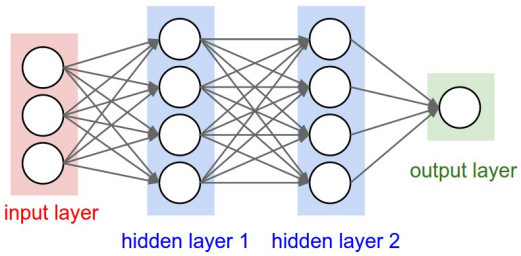
\includegraphics[scale=1]{feedforward.png}
  	\caption{An illustration \cite{hidden12} of a simple feed-forward neural network. It consists of four layers: an input layer (red), two hidden layers (blue) and one output layer (green). A circle represents a neuron. Every neuron in a layer is connected to all the neurons in the following layer, shown by the grey lines between the neurons. } \label{figfeedforward}
\end{figure}

A neuron is represented by a floating point decimal number. The value of a neuron is called its activation. Given an input of $n$ data points the model wants to predict $m$ different values. $n$ and $m$ are set as the size and number of neurons in the input and output layer respectively. The values of the input neurons are transferred to the next layer depending on the strength of the connection between every pair of neurons in two adjacent layers. This is done for every layer until the signal has reached the output layer. The process of propagating the value of the neurons from the input layer to the output layer is called forward propagation \cite{cs231n}.

The network is trained to predict correct values by optimizing the fixed connections, also called weights, between every pair of neurons in two consecutive layers in the neural network \cite{cs231n}.

\subsection{Tensors, indexing and notation}
A tensor is the generalization of vectors and matrices. Scalars are tensors of order 0. A tensor of order 1 is a row vector $x \in \mathbb{R}^N$ with $N$ elements. It can also be seen as a one-dimensional array. Matrices $M$ are tensors of order 2 such that $M \in \mathbb{R}^{R \times N}$ and can be viewed as vectors with $R$ elements where every element is another vector with $N$ scalar elements. Matrices can also be seen as a two-dimensional array with $RN$ elements. A tensor of order $n$ is an $n$-dimensional array and is indexed by an $n$-tuple. For instance, a tensor $X \in \mathbb{R}^{R \times C \times H \times W}$ is indexed by the four-tuple $(r,c,h,w)$ where $1 \leq r \leq R$, $1 \leq c \leq C$, $1 \leq h \leq H$ and $1 \leq w \leq W$ \cite{cs231n}.

\subsection{Forward propagation}
Figure \ref{figfeedforward} only illustrates a single set of input neurons, called a training example, being forward propagated. In practice a mini-batch of $R$ training examples is constructed and forward propagated at the same time \cite{cs231n} \cite{wikiStanford}.

Let $L$ denote the number of layers in the neural network and $l$, $1 \leq l \leq L$, one specific layer in the neural network. $N^{(l)}$ is the number of neurons in layer $l$. The activation (values) of layer $l$ can be expressed as a tensor of order 2: $X^{(l)} \in \mathbb{R}^{R \times N^{(l)}}$ indexed by the two-tuple $(r,i)$ where $1 \leq r \leq R$ and $1 \leq i \leq N^{(l)}$. In addition to the neurons of layer $l$, there is a bias neuron $b^{(l)} \in \mathbb{R}$ (see figure \ref{figFCCmath}). It is called a bias neuron because its value is independent to what input the neural network is given \cite{cs231n} \cite{wikiStanford}.

The weights representing the strength of the connections between the neurons of layer $l$ and $l+1$ are also expressed as a tensor of order 2. Let $W^{(l)} \in \mathbb{R}^{N^{(l+1)}  \times N^{(l)}}$ such that the element $W_{j, i}^{(l)}$ is the strength of the connection between neuron $X_{ri}^{(l)}$ and $X_{rj}^{(l+1)}$ for arbitrary example $r$ in the mini-batch \cite{cs231n} \cite{wikiStanford}.

\begin{figure}[h]
	\centering
  		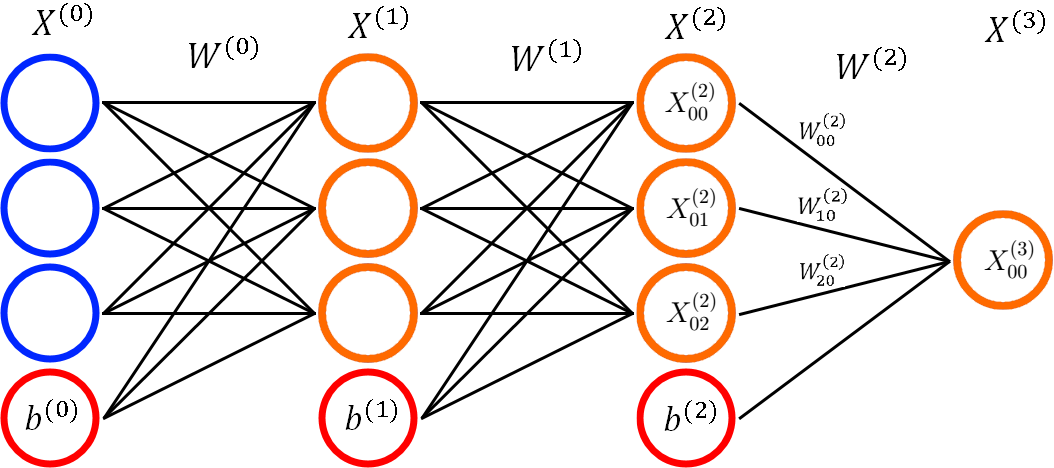
\includegraphics[scale=0.4]{FCC.png}
  	\caption{An example of a 4 layer feed-forward neural network. The input neurons are marked with blue. The bias neurons are marked with red. Black lines between neurons symbolyze the weights between every pair of neurons between two layers.} \label{figFCCmath}
\end{figure}

The calculation of the value of a neuron in layer $l+1$ includes computing the sum of every neuron in layer $l$ multiplied with its corresponding weight in $W^{(l)}$, plus the value of the bias $b^{(l)}$. The sum is then put in a so called activation function $f$. The value of the activation function is the neuron's activation in layer $l+1$ \cite{cs231n} \cite{wikiStanford}.

Let $Z^{(l)} \in \mathbb{R}^{R \times N^{(l)}}$ be the value of each neuron in layer $l$ before being put into the activation function. Given an input $X^{(1)}$ the forward propagation is expressed recursively as \cite{cs231n} \cite{wikiStanford}:

\begin{align}
Z_{rj}^{(l+1)} & = b^{(l)} + \sum^{N^{(l)}}_{i = 1} X^{(l)}_{r,i} W^{(l)}_{i,j}\\
X_{rj}^{(l+1)} & = f(Z_{rj}^{(l+1)})
\end{align}

The tensor of activations and weights are constructed in such a way that one forward pass through a single layer can be computed with a single dot product and an addition of the bias term added to every element. The activation function $f$ is then applied element-wise on each neuron \cite{cs231n} \cite{wikiStanford}:

\begin{align}
Z_{rj}^{(l+1)} & = \begin{bmatrix}
X^{(l)}W^{(l)}
\end{bmatrix}_{rj}+b^{(l)} \\
X_{rj}^{(l+1)} & = f(Z_{rj}^{(l+1)})
\end{align}

Common activation functions are Rectified Linear Units (ReLU), sigmoid ($\sigma$) and hyperbolic tangent ($\tanh$) and are defined by equations \eqref{relu} - \eqref{tanh} (see figure \ref{activation_function}). A non-linear activation function is chosen to enable the network to make use of non-linearities when learning to predict values. Without non-linear activation functions, the whole model is equivalent to one large linear transformation of the input data \cite{cs231n}.
\\
\begin{figure}[h]
	\centering
  		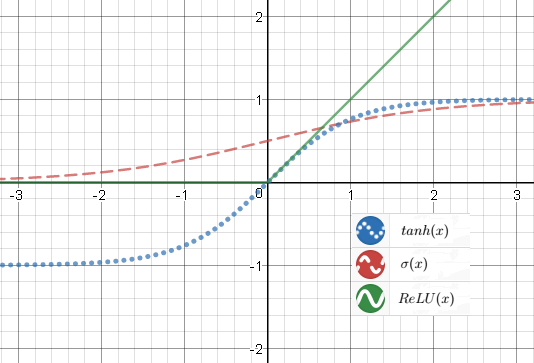
\includegraphics[scale=0.73]{activationfunction.png}
  	\caption{A graph of ReLU, $\sigma$ and $\tanh$.} \label{activation_function}
\end{figure}

\begin{equation}\label{relu}
\mbox{ReLU}{(x)} = \begin{cases} 
			0 & \mbox{if } x < 0 \\ 
			x & \mbox{if } x \geq 0 
		\end{cases}
\end{equation}

\begin{equation}\label{sigmoid}
\sigma(x) = \frac{1}{1+e^{-x}}
\end{equation}

\begin{equation}\label{tanh}
\tanh{(x)} = \frac{e^x-e^{-x}}{e^x+e^{-x}}
\end{equation}

\subsection{Loss function}
Given an input $X \in \mathbb{R}^{R \times N^{(1)}}$ and a ground truth $y \in \mathbb{R}^{R \times N^{(L)}}$ the model wants to predict values $\hat{y}$ which resembles the ground truth as closely as possible. It is achieved by defining a multivariate loss function $L(\theta; X, y)$  with the network's parameters $\theta$ (all the weights and biases) with respect to a single training mini-batch $(X, y)$. The loss function describes the quality of the neural network's prediction $\hat{y}$ such that a lower loss represents a more accurate prediction. $\hat{y}$ is synonymous with the activations of the last layer $L$ in the network and is a function of the parameters $\theta$ of the network and the input data $X$. $y$ is the human labeled ground truth with the same dimensionality as $\hat{y}$. To simplify noration $L(\theta)$ is used to denote the loss function with respect to one mini-batch $(X, y)$ of training data. One way of defining the loss function is to use the mean squared error defined by the following equation \cite{cs231n}:

\begin{equation}\label{MSE}
L(\theta) = \frac{1}{RN^{(L)}} \sum^{R}_{r=1} \sum^{N^{(L)}}_{i=1} (\hat{y}_{r,i}-y_{r,i})^2
\end{equation}

Here $R$ is the batch size and $N^{(L)}$ is the number of neurons in the last layer $L$.

The process of minimizing the loss function is called training. The model iterates through supervised training data and calculates the loss with respect to a mini-batch of training examples. Since the given input $X$ and ground truth $y$ stays fixed, the network learns by optimizing its weights $W^{(l)}$ and biases $b^{(l)}$ for every layer $l$ to decrease the loss \cite{cs231n} \cite{wikiStanford}.

\subsection{Gradient Descent}
The gradient $\nabla L(\theta)$ is a vector of partial derivatives with respect to the parameters $\theta$ of the function $L$ defined by the following equations \cite{gradient} \cite{convmath}:
\begin{equation}\label{EQgradientspace}
\nabla L(\theta) : \mathbb{R}^n \to \mathbb{R}^n
\end{equation}
\begin{equation}\label{EQgradientvector}
\nabla L(\theta) = 
	\begin{pmatrix} 
		\pd{L(\theta)}{\theta_{1}}, & 
		\pd{L(\theta)}{\theta_{2}}, &
		\cdots, &
		\pd{L(\theta)}{\theta_{n}}
		
		\end{pmatrix}
\end{equation}

The gradient $\nabla L(\theta)$ shows the direction of steepest ascent in the point ($\theta_{1}$, $\theta_{2}$, ..., $\theta_{n}$) in the $n$-dimensional vector space $\mathbb{R}^{n}$. For a function $f(x)$ of a single variable $x$, the gradient is simply the derivative of the function with respect to $x$ and is the slope of the tangent line to $f$ at $x$. For a function $f(x,y)$ of two variables $x$ and $y$, the gradient is the two-dimensional vector of the slope in the $x$ dimension and $y$ dimension respectively. The loss function used in neural networks can be a function of millions of parameters, depending on the depth and size of the neural network \cite{gradient} \cite{convmath}.

Gradient descent is the method of iteratively changing the values of the parameters $\theta$ proportionally to the negative gradient $-\nabla L(\theta)$ to minimize the function $L(\theta)$ (see figure \ref{figSGD}). The most basic algorithm of gradient descent is called Stochastic Gradient Descent (SGD) and uses the hyperparameter $\alpha$, called learning rate, to control the magnitude of the gradient. It is called Stochastic Gradient Descent because, at each iteration, the mini-batch responsible for the losses is randomly chosen and sampled from the whole batch of training data. Stochastic Gradient Descent is defined by the following equations \cite{wikiStanford} \cite{gradient} \cite{convmath}:

\begin{equation}\label{EQgradient}
\pd{L(\theta)}{\theta_i} = \nabla_{\theta_i} L(\theta)
\end{equation}
\begin{equation}\label{SGD}
{\theta_i} \to {\theta_i} - \alpha \pd{L(\theta)}{\theta_i}
\end{equation}

\begin{figure}[h]
	\centering
  		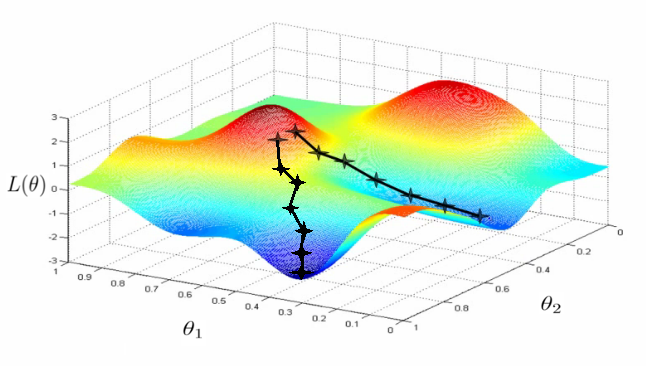
\includegraphics[scale=1]{gradient-descent.png}
  	\caption{An illustration \cite{figSGD} of Stochastic Gradient Descent on a function of two variables. Red regions symbolizes a high function value while blue regions symbolizes a low function value. The parameters were initialized near the global maximum and their values are altered iteratively to move in the direction of the negative gradient: the direction of steepest descent, to find a local minimum.} \label{figSGD}
\end{figure}

\subsection{Backpropagation}
Backpropagation is the process of calculating the partial derivatives of the loss function with respect to the model's parameters, or in other terms, the process of computing the gradient. The gradient is then used to modify the network's parameters to minimize the loss function \cite{wikiStanford} \cite{gradient}.

The partial derivatives can be approximated numerically with the formal definition of a derivative defined by the following equation \cite{wikiStanford} \cite{gradient}:

\begin{equation}\label{EQderivativeDefinition}
\pd{L(\theta)}{\theta_{i}} = \lim_{h \to 0} \frac{L(\theta_{1},...,\theta_{i} + h, ..., \theta_{n})-L(\theta)}{h}
\end{equation}

This would not be a problem for the small neural network in figure \ref{figFCCmath} with a total of 24 parameters, but would be extremely inefficient for deep neural networks with millions of parameters. Instead, the chain rule is applied to calculate the exact values of the partial derivatives in a computationally efficient manner \cite{cs231n}.

Let $\delta^{(l)}$ denote the so called delta-error at layer $l$, defined by the following equation:

\begin{equation}\label{deltaerrordefinition}
\delta^{(l)} = \inpd{L(\theta)}{X^{(l)}}
\end{equation}

The delta-error is the partial derivative of the loss with respect to a specific neuron in the model and is needed to efficiently compute the gradient with the help of the chain rule. The delta-error can be interpreted as how much a deviation in the value of a neuron affects the loss function. A change in value of a neuron with a big delta-error results in a greater change of the total loss compared to a neuron with a small delta-error. Because the activation of layer $l+1$ is a function of the previous layer $l$, the delta-error can be computed recursively from the output layer and propagated backwards to the first layer in the network. By applying the chain rule the delta-error $\inpd{L(\theta)}{X^{(l)}}$  at layer $l$ can be broken up into three partial derivatives $\inpd{L(\theta)}{X^{(l+1)}}$, $\inpd{X^{(l+1)}}{Z^{(l+1)}}$ and $\inpd{Z^{(l+1)}}{X^{(l)}}$. Since a single neuron in layer $l$ is connected to every neuron in layer $l+1$ you have to sum over every activation in layer $l+1$. The first partial derivative is the delta-error of the next layer and the other two partial derivatives are derived from equations (1) and (2) and are easily differentiable since (1) is a linear equation \cite{cs231n} \cite{wikiStanford}:
\begin{equation}\label{dLdX_FCC}
\begin{split}
\delta^{(l)}_{r,i}
	& = \pd{L(\theta)}{X^{(l)}_{r,i}}  \\
	& = \sum^{N^{(l+1)}}_{j=1} \pd{L(\theta)}{X^{(l+1)}_{r,j}} \pd{X^{(l+1)}_{r,j}}{Z^{(l+1)}_{r,j}} \pd{Z^{(l+1)}_{r,j}}{X^{(l)}_{r,i}} \\
	& = \sum^{N^{(l+1)}}_{j=1} \delta^{(l+1)}_{r,j} f'(Z^{(l+1)}_{r,i}) \ W^{(l)}_{j,i} 
\end{split}
\end{equation}

The delta-error of the last layer $L$ depends on the type of loss function used. For the mean squared error the delta-error of the output layer is defined by the following equation \cite{cs231n} \cite{wikiStanford}:

\begin{equation}\label{MSEdelta}
\begin{split}
\delta^{(L)}
	& = \pd{L(\theta)}{\hat{y}}  \\
	& = \frac{2}{RN^{(L)}} (\hat{y}-y)
\end{split}
\end{equation}

With the delta-error defined at every layer in the network the partial derivative of the loss function with respect to the networks parameters can be calculated. Just like equation (\ref{dLdX_FCC}), the chain rule is applied to break up $\inpd{L(\theta)}{X^{(l)}}$ into three partial derivatives, $\inpd{L(\theta)}{X^{(l+1)}}$, $\inpd{X^{(l+1)}}{Z^{(l+1)}}$ and $\inpd{Z^{(l+1)}}{W^{(l)}}$. All the examples in the mini-batch are summed over since the weights affect every single example. $\inpd{L(\theta)}{X^{(l+1)}}$ is the delta-error and the other two partial derivatives are derived from equations (1) and (2) \cite{cs231n} \cite{wikiStanford}:

\begin{equation}\label{dLdW_FCC}
\begin{split}
\pd{L(\theta)}{W^{(l)}_{j,i}} 
	& = \sum^{R}_{r=1} \pd{L(\theta)}{X^{(l+1)}_{r,i}} \pd{X^{(l+1)}_{r,i}}{Z^{(l+1)}_{r,i}} \pd{Z^{(l+1)}_{r,i}}{W^{(l)}_{i,j}} \\
	& = \sum^{R}_{r=1} \delta^{(l+1)}_{r,i} f'(Z^{(l+1)}_{r,i}) \ X^{(l)}_{r,j}\\
\end{split}
\end{equation}

The partial derivative of the loss function with respect to the biases are found in a similar way to equations (\ref{dLdX_FCC}) and (\ref{dLdW_FCC}) \cite{cs231n} \cite{wikiStanford}:
\begin{equation}\label{dLdb_FCC}
\begin{split}
\pd{L(\theta)}{b^{(l)}} 
	& = \sum^{R}_{r=1} \pd{L(\theta)}{X^{(l+1)}_{r,i}} \pd{X^{(l+1)}_{r,i}}{Z^{(l+1)}_{r,i}} \pd{Z^{(l+1)}_{r,i}}{b^{(l)}_{i,j}} \\
	& = \sum^{R}_{r=1} \delta^{(l+1)}_{r,i} f'(Z^{(l+1)}_{r,i}) \\
\end{split}
\end{equation}

\subsection{Training neural networks}
The model is trained by dividing the training data into mini-batches of size $R$. A mini-batch is then forward propagated and the loss is calculated. The loss is then used to backpropagate the model's deviation from the ground truth (the network's loss) layer by layer. Backpropagation starts at the output layer and propagates through the network backwards until it reaches the input layer. For every layer in the network the delta-error from the proceeding layer is used to calculate the new delta-error. It is then used to calculate the layers contribution to the total gradient by computing the partial derivatives with respect to the loss function. When the gradient has been fully computed, one iteration of the gradient descent algorithm is applied to update the weights and biases of the neural network. This process is repeated until all the networks parameters have converged \cite{cs231n}.

Two implementations of a feed-forward neural network can be found on github in Python and C++ in the repositories \textit{neural-network-python} and \textit{neural-network-cpp} respectively: \url{https://github.com/nikitazozoulenko}.

\section{Convolutional neural networks}
When humans identify objects by sight we look for specific high level features that object has. A cat for example has one head, four legs and a body. These high level features are in turn made up of a combination of low level features: A head consists of two eyes and a mouth which consists of elementary geometric shapes which are composed of a combination of basic lines and edges. In addition to specific features, cats also have a furry texture. Convolutional neural networks (CNN) were designed to specifically excel at computer vision tasks. What a convolutional neural network does is that it learns these hierarchical structures by teaching itself a number of filters to apply to the image (see figure \ref{figkatter}) through an operation called a convolution. These filters are stacked on top of each other in terms of layers and allows the networks to learn higher level features with the network architecture going deeper. For instance, the first layer might learn how to detect lines and edges, the middle layers might learn to recognize small body parts such as eyes and ears and the last layers can learn how to detect cats, humans or any other arbitrary objects \cite{cs231n}.

\begin{figure}[h]
	\centering
  		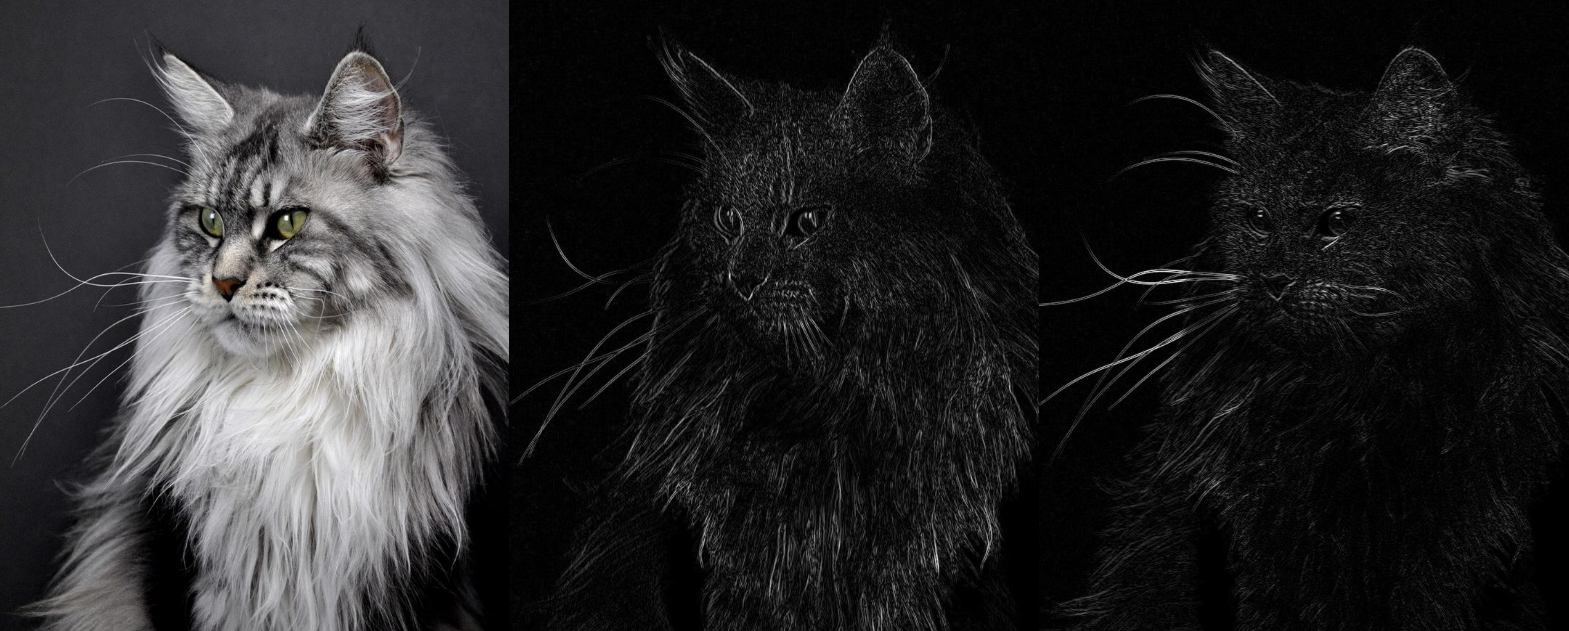
\includegraphics[scale=0.33]{katter.png}
  	\caption{The result of a filter for vertical and horizontal edge detection applied on a picture of a cat.} \label{figkatter}
\end{figure}

In feed-forward neural networks every neuron in a layer is connected to all the neuron in the next layer. If you would use feed-forward neural networks for a computer vision problem you would reshape the given input image to a single $CHW$-dimensional vector where $W$ and $H$ are the images width and height in pixels and $C$ is the number of color channels in the image. Because every neuron in the previous layer is connected to all the neurons in the proceeding layer most of the spatial information in the image is lost. Convolutional neural networks are different in the way how they operate on spatially local data. The neurons in layer $l$ are only connected to the neurons in layer $l+1$ that are in the close spatial vicinity of the neurons in layer $l$. In practice this has yielded more accurate predictions over their feed-forward counterparts and has lead to the model becoming the state of the art in computer vision \cite{cs231n} \cite{convmath} \cite{convarithmetic}.

\subsection{Model structure, parameters and notation}
Convolutional neural networks are composed of a number of layers stacked on top of each other, similar to feed-forward neural networks. The difference between these two models is how one layer is connected to the next layer. While feed-forward neural networks have only one type of layer, convolutional neural networks have a wide variety of different layers. The five elementary layers and operations of the convolutional neural network are the convolutional layer, the maxpooling layer, the softmax layer, the activation function layer and batch normalization, which all behave differently. A convolutional neural network can also use fully connected layers where every neuron in a layer $l$ is connected to all neurons in layer $l+1$, which behave exactly the same as feed-forward neural networks \cite{cs231n} \cite{convmath} \cite{convarithmetic}.

At every layer $l$ there are parameters $\theta^{(l)}$ and activations (neurons) $X^{(l)}$. The last layer is characterized by $\hat{y}$ and $X^{(L)}$ where $L$ is the number of layers in the network. Given an input $X^{(1)}$ the model predicts values $\hat{y}$. The input is forward propagated recursively by using the activations $X^{(l)}$ and parameters $\theta^{(l)}$ from layer $l$ to compute the activations in layer $l+1$, defined by equation \eqref{CNNeq}. Simiar to feed-forward neural network, the prediction is then put into a loss function $L(\theta)$, which is used by the backpropagation algorithm along with Stochastic Gradient Descent to train the network \cite{cs231n} \cite{convmath}.

\begin{equation}\label{CNNeq}
X^{(1)} \xrightarrow{\theta^{(1)}} X^{(2)}  \xrightarrow{\theta^{(2)}} \cdots  \xrightarrow{\theta^{(L-2)}} X^{(L-1)}  \xrightarrow{\theta^{(L-1)}} X^{(L)} = \hat{y}
\end{equation}

To be able to fully utilize the spatial information from a given input the model represent the activation at a given layer $l$ as a tensor of order 4: $X^{(l)} \in \mathbb{R}^{R \times C  \times H \times W}$. A layer takes in a batch of three-dimensional volumes of neurons and produces a new batch of three-dimensional volumes of neurons at the next layer. $R$ stands for the batch size and $C$, $W$ and $H$ are the depth, width and and height of the volume of neurons. To feed an image into the model, the image is made into a tensor of size $3 \times H \times W$ where the values of the neurons are the value of the pixels in the image, for all 3 red, green and blue color channels in the image. The image tensors are then stacked into a single tensor of size $R \times 3 \times H \times W$ to form a mini-batch \cite{cs231n}.

A $H \times W$ slice of the activations is called a feature map or a channel. Convolutional neural networks are usually illustrated as three-dimensional volumes of activations (see figure \ref{figvgg}) or as stacked feature maps (see figure \ref{figboatcnn}) \cite{cs231n} \cite{convmath} \cite{convarithmetic}. 

\begin{figure}[h]
	\centering
  		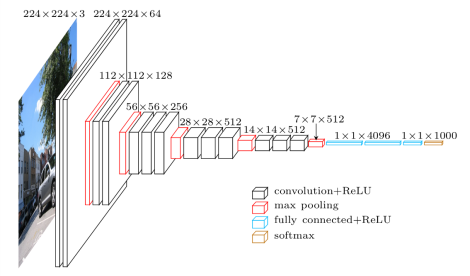
\includegraphics[scale=0.6]{vggnet.png}
  	\caption{An illustration \cite{vgg} of a the VGGNet19 convolutional neural network. The different volumes represent the activations of the network at different depths. Each two-dimensional slice is a feature map.} \label{figvgg}
\end{figure}

\begin{figure}[h]
	\centering
  		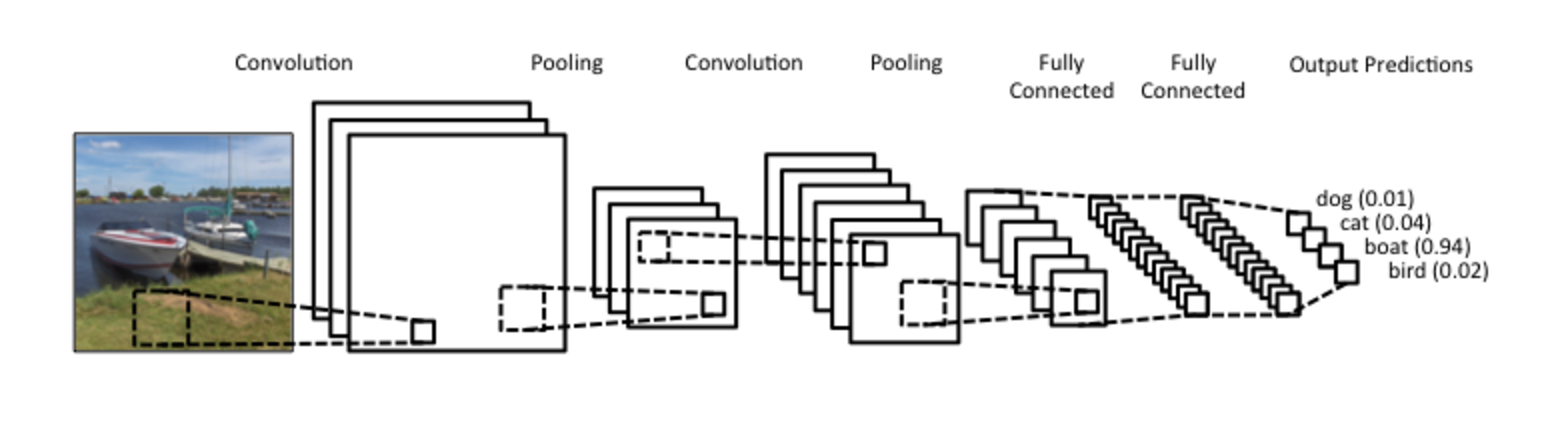
\includegraphics[scale=0.6]{boatcnn.png}
  	\caption{An illustration \cite{figkonv} of a convolutional neural network. Each two-dimensional slice is a feature map.}\label{figboatcnn}
\end{figure}

Every single type of layer in a convolutional neural network has two modes: forward propagation and backpropagation. The model is trained the same way as a feed-forward neural network is trained: A given input is forward propagated to get a loss which is then backpropageted though the network. Thus, for every layer there has to be a definition of forward propagation and backpropagation. In the forward propagation the activations from the previous layer are used to calculate the activations in the next layer. During backpropagation the delta-error from the next layer is used to calculate the delta-error of the previous layer. The delta-error is then used to compute the partial derivatives needed for the gradient \cite{cs231n} \cite{convmath}. 

Because every layer operation in the neural network is defined sequentially, we only have to define operations for two adjacent layers. Let the size of the tensor of activations at layer $l$ have size $R \times C \times H \times W$. At the next layer, $l+1$, the activations will be of size $R \times C' \times H' \times W'$. The prime notation specifies that the variable originates from the proceeding layer and is the same for the indices. The tensors are indexed by the four-tuple $(r, c, h, w)$. The batch size always stays the same from layer to layer, while the spatial size can decrease depending on the layer type \cite{cs231n} \cite{convmath}. 

\subsection{Convolution forward propagation}
The basic building block of the convolutional neural network is the convolution and the convolutional layer. It uses the learnable parameters $W^{(l)} \in \mathbb{R}^{C' \times C  \times k \times k}$, called a kernel, and is the before mentioned filter the network learns to apply to images. $C$ and $C'$ are the number of channels in layer $l$ and $l+1$ respectively. $k$ is a variable called the kernel size of the convolution \cite{cs231n}. 

The activations at layer $l+1$ are derived from the activations at layer $l$ by applying the kernel at every possible spatial location on the activations at layer $l$ (see figure \ref{figkonv}). Every neuron is multiplied by the value of the kernel at the same spatial location. The sum of all the products becomes the activation of a single neuron in layer $l+1$. Applying this operation on every region of neurons in the activation is called a convolution. The convolution operator is denoted by $*$ \cite{cs231n} \cite{convmath} \cite{convarithmetic}. 

\begin{figure}[h]
	\centering
  		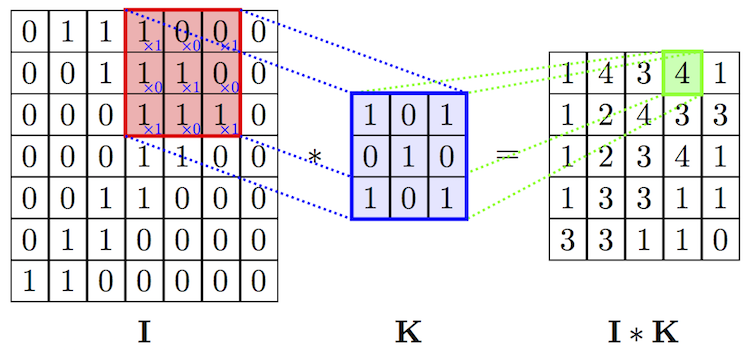
\includegraphics[scale=2.1]{convolution.png}
  	\caption{A kernel of size $1 \times 3 \times 3$ convolving over activations of size $1 \times 7 \times 7$, producing activations of size $1 \times 4 \times 4$ in the next layer \cite{figconv}. } \label{figkonv}
\end{figure}

A feature map in layer $l+1$ is the result of a single kernel of size $1 \times C  \times k\times k$ being convolved over the whole activation volume of the previous layer. $C'$ is the number of kernels a layer has and is also the number of feature maps the next layer will have \cite{cs231n} \cite{convmath}. 

The kernels have two additional non-learnable hyperparameters: a stride $s$ and zero-padding $p$. $s$ is the size of the step the kernel takes when it moves from one spatial location to the next during a convolution. The convolution in figure \ref{figkonv} has a stride of $s = 1$. Zero-padding entails padding the edges of the activation tensor with $p$ zeros (see figure \ref{figzeropad}). Since a convolution decreases the spatial size of the activations of the next layer, zero-padding is a way to control the size of the activations \cite{cs231n} \cite{convmath} \cite{convarithmetic}. 

\begin{figure}[h]
	\centering
  		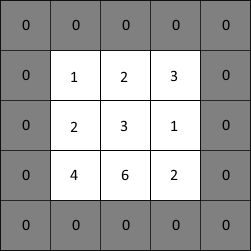
\includegraphics[scale=0.7]{zeropadding.png}
  	\caption{An activation with size $1 \times 3 \times 3$ is zero-padded with $p=1$ and the resulting tensor is of size $1 \times 5 \times 5$. White symbolizes the original tensor and grey symbolizes the padded zeros. } \label{figzeropad}
\end{figure}

Let $W^{(l)} \in \mathbb{R}^{C' \times C  \times k \times k}$, $X^{(l)} \in \mathbb{R}^{R \times C  \times (H+2p) \times (W+2p)}$ and $X^{(l+1)} \in \mathbb{R}^{R \times C'  \times H' \times W'}$. The dimensions of layer $l+1$ are defiend by equations \eqref{eqkonvW} and \eqref{eqkonvH} \cite{cs231n} \cite{convmath} \cite{convarithmetic}: 
\begin{equation}\label{eqkonvW}
W' = \frac{W-k+2p}{s} +1
\end{equation}
\begin{equation}\label{eqkonvH}
H' = \frac{H-k+2p}{s} +1
\end{equation}
The following equation defines the convolutional layer algebraically \cite{cs231n} \cite{convmath}:
\begin{equation}
w = sw'
\end{equation}
\begin{equation}
h = sh'
\end{equation}
\begin{equation}\label{konvolution}
\begin{split}
	\begin{bmatrix} X^{(l+1)} \end{bmatrix}_{r, c', h', w'}	
		& = X^{(l)}_{r, c', h', w'} *W^{(l)}_{c'} \\
		& = \sum^{C}_{c=1} \sum^{k}_{j=1} \sum^{k}_{i=1} X^{(l)}_{r, c, h'+j, w'+i}W^{(l)}_{c', c, j, i}
\end{split}
\end{equation}

The index of the term which shall be used to convolve specifies which dimensions will be convolved upon and summed over. For instance, $W^{(l)}_{c'}$ implies that the $C$, $H$ and $W$ dimensions (all channels) should be used in the convolution, while $W^{(l)}_{c', c}$ implies that only the $H$ and $W$ dimension (one channel) should undergo the convolution operation.

Convolutions are in practice implemented with the functions $row2im$ and $im2row$ which enable the convolution to be computed with a single dot product \cite{cs231n} \cite{convmath} \cite{convarithmetic}. The underlying math is equivalent with the equations shown in this paper. However, $row2im$ and $im2row$ are outside of the scope of this paper and are left to the reader to research if a more computationally efficient implementation is required. 

\subsection{Convolution backpropagation}
At every layer $l$ the delta-error of the proceeding layer $\delta^{(l+1)}$ has to be backpropagated to create the delta-error at the current layer. $\delta^{(l)}$ is then used to compute the partial derivatives of the loss with respect to the weights $W^{(l)}$ to be used in the gradient \cite{cs231n} \cite{convmath}. 
 
The backpropagation of the recursive delta-error $\delta^{(l+1)}$ is derived by the use of the chain rule. $\delta^{(l+1)} = \inpd{L(\theta)}{X^{(l+1)}}$ is broken up into two smaller partial derivatives $\inpd{L(\theta)}{X^{(l+1)}}$ and $\inpd{X^{(l+1)}}{X^{(l)}}$. Additionally, because more than one single neuron in layer $l$ is responsible for the delta-error at layer $l+1$, all the neurons of layer $l$ have to be summed over, similar to equation \eqref{dLdX_FCC}, \eqref{dLdW_FCC}, and \eqref{dLdb_FCC}. This can be done since the derivative of a sum is equivalent to the sum of the derivatives of each element. $X^{(l+1)}_{r,c',h',w'}$ is then replaced by its definition from equation \eqref{konvolution} \cite{convmath} \cite{webconv1} \cite{webconv2} \cite{webconv3}: 

\begin{equation}\label{konvolutionbackprop}
\begin{split}
	\delta^{(l)}_{r,c,h,w}
		& = \pd{L(\theta)}{X^{(l)}_{r,c,h,w}} \\
		& = \sum^{C' }_{c'=1} \sum^{H' }_{h'=1} \sum^{W' }_{w'=1} \pd{L(\theta)}{X^{(l+1)}_{r,c',h',w'}} \pd{X^{(l+1)}_{r,c',h',w'}}{X^{(l)}_{r,c,h,w}} \\
		& = \sum^{C' }_{c'=1} \sum^{H' }_{h'=1} \sum^{W' }_{w'=1} \delta^{(l+1)}_{r,c',h',w'} \pd{\sum^{C }_{c=1} \sum^{k }_{j=1} \sum^{k }_{i=1} X^{(l)}_{r, c, h'+j, w'+i}W^{(l+1)}_{c', c, j, i}}{X^{(l)}_{r,c,h,w}}
\end{split}
\end{equation}

Every partial derivative in the most inner sum will be equal to to zero if $X^{(l)}_{r, c, h'+j, w'+i} \neq X^{(l)}_{r,c,h,w}$. Using the substitutions $h = h'+j$ and $w = w'+i$ the three inner sums are cancelled out \cite{webconv1} \cite{webconv2} \cite{webconv3}:

\begin{multline}
\sum^{C' }_{c'} \sum^{H' }_{h'=1} \sum^{W' }_{w'=1} \delta^{(l+1)}_{r,c',h',w'} \pd{\sum^{C }_{c=1} \sum^{k }_{j=1} \sum^{k }_{i=1} X^{(l)}_{r, c, h'+j, w'+i}W^{(l+1)}_{c', c, j, i}}{X^{(l)}_{r,c,h,w}} \\
	 = \sum^{C' }_{c'=1} \sum^{H' }_{h'=1} \sum^{W' }_{w'=1} \delta^{(l+1)}_{r,c',h',w'} W^{(l+1)}_{c', c, (h-h'), (w-w')}     \\
\end{multline}

Which one can see is a sum of convolutions where a feature map of the delta-error of layer $l+1$ convolves over all the kernels of layer $l$ where the kernels are rotated by $180^\circ$. This is intuitive since every feature map in $X^{(l)}$ is used to create a single feature map in $X^{(l+1)}$. Let the rotation of the kernel be denoted with the function $rot()$. The final equation of the backpropagation of the delta-error is defined by the following equation \cite{webconv1} \cite{webconv2} \cite{webconv3}: 
\begin{equation}\label{eqconvfinal}
\delta^{(l)}_{r,c,h,w} = \sum^{C' }_{c'=1} rot(W^{(l+1)}_{c',c,h,w}) * \delta^{(l+1)}_{r,c'}
\end{equation}

The partial derivative of the loss $L(\theta)$ with respect to the weights $W^{(l)}$ is derived the same way the backpropagation of the error is derived. The only change is that the $R$-dimension is summed over since every example in the mini-batch is a function of the loss, and affects the gradient \cite{cs231n} \cite{webconv1} \cite{webconv2} \cite{webconv3}. 
\begin{align}
\begin{split}
	\pd{L(\theta)}{W^{(l)}_{c',c,h,w}}
		& = \sum^{R }_{r=1} \sum^{C' }_{c'=1} \sum^{H' }_{h'=1} \sum^{W' }_{w'=1} \pd{L(\theta)}{X^{(l+1)}_{r,c',h',w'}} \pd{X^{(l+1)}_{r,c',h',w'}}{W^{(l)}_{r,c,h,w}} \\
		& = \sum^{R }_{r=1} \sum_{c'=1}^{C' } \sum^{H' }_{h'=1} \sum^{W' }_{w'=1} \delta^{(l+1)}_{r,c',h',w'} \pd{\sum\limits^{C }_{c=1} \sum\limits^{k }_{j=1} \sum\limits^{k}_{i=1} X^{(l)}_{r, c, h'+j, w'+i}W^{(l)}_{c', c, j, i}}{W^{(l)}_{c',c,h,w}} \\
		& = \sum^{R }_{r=1} \sum^{C' }_{c'=1} \sum^{H' }_{h'=1} \sum^{W' }_{w'=1} X^{(l)}_{r, c, h'+h, w'+w} \delta^{(l+1)}_{r,c',h',w'} \\
		& = \sum^{R }_{r=1} \sum^{C' }_{c'=1} X^{(l)}_{r, c, h, w} * \delta^{(l+1)}_{r,c'} \\
\end{split}
\end{align}

\subsection{Activation function forward propagation}
In the activation function layer an activation function $f$ is applied element wise on every neuron in the activation tensor. Thus, the size of $X^{(l)}$ and $X^{(l+1)}$ is the same. Any differentiable function can be used as an activation function, but the most commonly used ones are ReLU, sigmoid and $\tanh$. The activation function layer does not have any learnable parameters. Activation functions enable the network to learn faster while also increasing the accuracy of the predictions \cite{cs231n} \cite{convmath}. 
 
Forward propagation is defined by:
\begin{equation}\label{eqactivation}
X^{(l+1)}_{r,c,h,w} = f(X^{(l)}_{r,c,h,w})
\end{equation}

\subsection{Activation function backpropagation}
Because the activation function layer does not have any learnable parameters only the recursive delta-error has to be backpropagated. It is derived by the use of the chain rule. $\inpd{L(\theta)}{X^{(l)}}$ is split up into $\inpd{L(\theta)}{X^{(l+1)}}$ and $\inpd{X^{(l+1)}}{X^{(l)}}$. The first term is simply the delta-error of the proceeding layer and the second term is the derivative of the activation function \cite{cs231n} \cite{convmath}: 

\begin{equation}
\begin{split}
\delta^{(l)}_{r,c,h,w}
		& = \pd{L(\theta)}{X^{(l)}_{r,c,h,w}} \\
		& = \pd{L(\theta)}{X^{(l+1)}_{r,c,h,w}} \pd{X^{(l+1)}_{r,c,h,w}}{X^{(l)}_{r,c,h,w}} \\
		& = \delta^{(l+1)}_{r,c,h,w} f'(X^{(l)}_{r,c,h,w})
\end{split}
\end{equation}

\subsection{Maxpooling forward propagation}
Maxpooling is a way to reduce the spatial size of the activations from one layer to the next. Every feature map in layer $l$ is divided into a number of regions of size $k \times k$ where $k$ is the hyperparameter called kernel size. One single $k \times k$ region corresponds to a single activation in the proceeding layer $l+1$. The activation is given by the maximum value of the region (see figure \ref{figmaxpool}). Additionally, maxpooling also has the hyperparameter $s$, called its stride, and works similar to the stride for the convolutional layer. $s$ denotes the step size that the $k \times k$ region uses when it traverses the volume of activations. Maxpooling does not have any learnable parameters \cite{cs231n} \cite{convmath} \cite{convarithmetic}. 

\begin{figure}[h]
	\centering
  		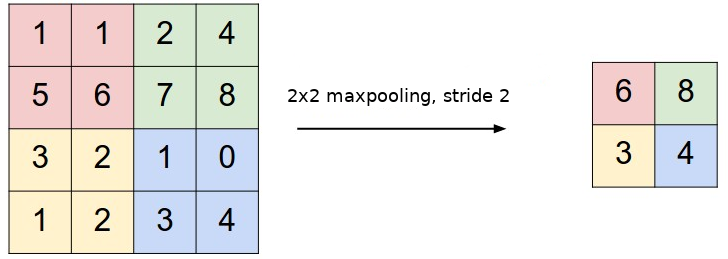
\includegraphics[scale=0.7]{maxpool.png}
  	\caption{Maxpooling with kernel size $k=2$ and stride $s=2$ on an area of size $4 \times 4$. The resulting area has size $2 \times 2$ \cite{figkonv}} \label{figmaxpool}
\end{figure}

Similar to a convolution without zero-padding, the dimensions of the proceeding layer is defined by the following equations. The number of feature maps remain constant \cite{cs231n} \cite{convmath} \cite{convarithmetic}: 
\begin{equation}
W' = \frac{W-k}{s}+1
\end{equation}
\begin{equation}
H' = \frac{H-k}{s}+1
\end{equation}
\begin{equation}
C' = C
\end{equation}

The following equation defines the maxpooling layer algebraically \cite{cs231n} \cite{convmath}:
\begin{equation}\label{maxpool}
X^{(l+1)}_{r,c',h',w'} = \underset{0 \leq j < k, \ 0 \leq i < k}{\max} X^{(l)}_{r,c',(h's+j),(w's+i)}
\end{equation}

\subsection{Maxpooling backpropagation}
Maxpooling does not have any learnable parameters and thus only the recursive delta-error has to be backpropagated. With the use of the chain rule the delta-error at layer $l$ is split into two partial derivatives $\inpd{L(\theta)}{X^{(l+1)}}$ and $\inpd{X^{(l+1)}}{X^{(l)}}$. The first term is the delta-error at layer $l+1$. $X^{(l+1)}$ is then substituted with its definition from equation \eqref{maxpool} \cite{cs231n} \cite{convmath} \cite{webconv3}: 

\begin{equation}
\begin{split}
	\delta^{(l)}_{r,c,h,w}
		& = \pd{L(\theta)}{X^{(l)}_{r,c,h,w}} \\
		& = \pd{L(\theta)}{X^{(l+1)}_{r,c',h',w'}} \pd{X^{(l+1)}_{r,c',h',w'}}{X^{(l)}_{r,c,h,w}} \\
		& = \delta_{r,c',h',w'} \pd{\underset{0 \leq j < k,0 \leq i < k}{\max} X^{(l)}_{r,c',(h's+j),(w's+i)}}{X^{(l)}_{r,c,h,w}} \\
\end{split}
\end{equation}

The partial derivative in the last equation will be equal to 1 if and only if $X^{(l)}_{r,c',(h's+j),(w's+i)} = X^{(l)}_{r,c,h,w}$. For any other case $X^{(l)}_{r,c,h,w}$ will not have any effect on the neurons in the proceeding layer $l+1$ and the partial derivative will thus be equal to 0 \cite{cs231n} \cite{convmath} \cite{webconv3}:
\begin{equation}
\delta^{(l)}_{r,c,h,w} = \begin{cases}
				\delta_{r,c,h',w'} & \mbox{if } \begin{split} h = h's+j, \\w = w's+i \end{split}\\
				0 & \mbox{otherwise}\\
			\end{cases}
\end{equation}

The delta-error from layer $l+1$ is thus redirected to the neuron in layer $l$ that is responsible for the activation which the delta error at layer $l+1$ corresponds to. If a neuron in layer $l$ is responsible for two or more activations in layer $l+1$ its delta error will become the sum of the delta-errors of the activations in question \cite{cs231n} \cite{convmath} \cite{webconv3}. 

\subsection{Batch Normalization forwardpropagation}
Neural networks are hard to train because of their recursive nature. A small change in the weights of the first layer will have a cascading effect throughout the network: The changed second layer will create a slightly larger deviation in the third layer, and the change in the third layer will have an even bigger effect on the fourth layer, and so on. One small change in the first layers can have a dramatic effect on the final prediction of the neural network. This is called  the internal covariate shift in the litterature and is what Batch Normalization (BN) sets out to fix \cite{cs231n} \cite{batchnorm}. 

Batch Normalization normalizes every feature map by dividing the feature map with the variance of the whole mini-batch's variance at the specified feature map, and subtracting the mean of the whole mini-batch's feature map. The cascading effect of a change in the first layer causing a bigger change in the last layers will no longer take place since every layer aims to have a variance of 1 and mean of 0. The internal covatiate shift is thus minimized \cite{cs231n} \cite{batchnorm}. 

To derive the activations at layer $l+1$ the mean and variance of every feature map in layer $l$ has to be computed. Let $\mu_c$ and $\sigma^2_c$ be the mean and variance of the feature map $c$ defined by the following equations \cite{cs231n} \cite{batchnorm}: 
\begin{equation}\label{eqmuc}
\mu_c = \frac{1}{RHW} \sum^{R }_{r=1} \sum^{H }_{h=1} \sum^{W }_{w=1} X^{(l)}_{r,c,h,w}
\end{equation}
\begin{equation}\label{eqsigmac}
\sigma^2_c  = \frac{1}{RHW} \sum^{R }_{r=1} \sum^{H }_{h=1} \sum^{W }_{w=1} ({X^{(l)}_{r,c,h,w} - \mu_c})^2
\end{equation}
Let $\hat{X}$ denote the normalized activations \cite{cs231n} \cite{batchnorm}. It is defined by:
\begin{equation}\label{xhat}
\hat{X}_{r,c,h,w} = (X^{(l)}_{r,c,h,w} - \mu_c){(\sigma^2_c)}^{-\frac{1}{2}}
\end{equation}

The normalized activations are then transformed by an affine transformation with the learnable parameters $\gamma_{c}^{(l)}$ and $\beta_{c}^{(l)}$. They enable the network to undo the normalization from equation \eqref{xhat} if the network deems it will result in more accurate predictions. The final activations at layer $l+1$ is defined by the following equation \cite{cs231n} \cite{batchnorm}:
\begin{equation}\label{eqbn}
X^{(l+1)}_{r,c,h,w} = \gamma_{c}^{(l)} \hat{X}_{r,c,h,w} + \beta_{c}^{(l)}
\end{equation}

When the network is used for predictions outside of the training, also called runtime, the network cannot calculate the needed statistics of the mini-batch to perform forward propagation since a batch size of 1 is usually used at runtime. To combat this, the statistics of the whole training data can be used to approximate the mean and variance of the activations. This can be done for small datasets, but is inpractical for training data with millions of examples. Instead, an exponentially weighted moving average which is updated at every forward propagation can be used to approximate the mean and variance of the whole population \cite{cs231n} \cite{batchnorm}. 

Let $\mu_{EWMA_c}$ and $\sigma^2_{EWMA_c}$ denote the exponentially weighted moving average for the mean and variance of the feature map $c$. Let $\lambda$ be the weight decay term. The moving averages are then defined by the following equations:

\begin{equation}\label{eqewmamu}
\mu_{EWMA_c} \to \lambda \mu_c + (1-\lambda)\mu_{EWMA_c}
\end{equation}
\begin{equation}\label{eqewmasigma}
\sigma^2_{EWMA_c} \to \lambda \sigma^2_c + (1-\lambda)\sigma^2_{EWMA_c}
\end{equation}

\subsection{Batch Normalization backpropagation}
At every layer $l$ the delta-error of the previous layer $\delta^{(l+1)}$ has to be backpropagated to create the delta-error at the current layer. The delta-error is then used to compute the partial derivatives of the loss with respect to the learnable parameters $\gamma_{c}^{(l)}$ and $\beta{c}^{(l)}$ to be used in the gradient. To aid the derivation of the backpropagation the kronecker-delta $I$ is used. The kronecker-delta has the following properties \cite{webBN1} \cite{webBN2}: 
\begin{equation}\label{kroneckerdelta}
I_{i,j} = \begin{cases} 1 & \mbox{if } i = j \\ 0 & \mbox{if } i \neq j  \end{cases}
\end{equation}
\begin{equation}\label{kroneckerdeltaDERIVATIVE}
\pd{a_{j}}{a_i} = I_{i,j}
\end{equation}
\begin{equation}\label{kroneckerdeltaSUM}
\sum_j  a_i  I_{i,j} = a_j
\end{equation}

The backpropagation of the recursive delta-error $\delta^{(l+1)}$ is derived by the use of the chain rule. $\inpd{L(\theta)}{X^{(l)}}$ is broken up into three partial derivatives and the sum of all the neurons is taken, similar to equation \eqref{konvolutionbackprop}. Additionally, the $R$-dimension is summed over since every example in the mini-batch has an effect on a single neuron in proceeding layer \cite{webBN1} \cite{webBN2}. 
\begin{align}\label{BN_delta_error}
\begin{split}
	\delta^{(l)}_{r,c,h,w}
		& = \pd{L(\theta)}{X^{(l)}_{r,c,h,w}} \\
		& = \sum^{R' }_{r'=1} \sum^{C' }_{c'=1} \sum^{H' }_{h'=1} \sum^{W' }_{w'=1} \pd{L(\theta)}{X^{(l+1)}_{r',c',h',w'}} \pd{X^{(l+1)}_{r',c',h',w'}}{\hat{X}_{r',c',h',w'}} \pd{\hat{X}_{r',c',h',w'}}{{X}^{(l)}_{r,c,h,w}}\\
\end{split}
\end{align}
$\inpd{L(\theta)}{X^{(l+1)}}$ is the delta-error of the proceeding layer. $\inpd{X^{(l+1)}}{\hat{X}}$ is easily differentiable since equation \eqref{eqbn} is a linear equation \cite{webBN1} \cite{webBN2}.

\begin{equation}\label{BN_dxdxhat}
\begin{split}
	\pd{X^{(l+1)}_{r',c',h',w'}}{\hat{X}_{r',c',h',w'}}
		& = \pd{(\gamma_{c'}^{(l)} \hat{X}_{r',c',h',w'} + \beta_{c'}^{(l)})}{\hat{X}_{r',c',h',w'}} \\
		& =\gamma_{c'}^{(l)}
\end{split}
\end{equation}

The partial derivative of the normalized activations $\hat{X}$ with respect to the activations $X^{(l)}$ is derived by substituting $X^{(l)}$ with its definition from equation \eqref{xhat} and then using the product rule \cite{webBN1} \cite{webBN2}: 
\begin{equation}\label{BN_kedjeregeln}
\begin{split}
\pd{\hat{X}_{r',c',h',w'}}{{X}^{(l)}_{r,c,h,w}} 
	& = \pd{(X^{(l)}_{r',c',h',w'} - \mu_{c'}){(\sigma^2_{c'})}^{-\frac{1}{2}}}{{X}^{(l)}_{r,c,h,w}} \\
	& = {(\sigma^2_{c'})}^{-\frac{1}{2}} \pd{(X^{(l)}_{r',c',h',w'} - \mu_{c'})}{{X}^{(l)}_{r,c,h,w}} - \frac{1}{2}(X^{(l)}_{r',c',h',w'} - \mu_c){(\sigma^2_{c'})}^{-\frac{3}{2}} \pd{\sigma^2_{c'}}{{X}^{(l)}_{r,c,h,w}}
\end{split}
\end{equation}

The derivative of the first factor with respect to the activation is derived by substituting the batch mean $\mu_{c'}$ with its definition from equation \eqref{eqmuc} and then using the kronecker-delta from equations \eqref{kroneckerdelta}, \eqref{kroneckerdeltaDERIVATIVE} and \eqref{kroneckerdeltaSUM} \cite{webBN1} \cite{webBN2}: 
\begin{equation}\label{mu'}
\begin{split}
\pd{(X^{(l)}_{r',c',h',w'} - \mu_{c'})}{{X}^{(l)}_{r,c,h,w}}
	& = \pd{({X^{(l)}_{r',c',h',w'} - \frac{1}{RHW} \sum\limits^{R }_{r''=1} \sum\limits^{H }_{h''=1} \sum\limits^{W }_{w''=1} X^{(l)}_{r'',c',h'',w''}})}{{X}^{(l)}_{r,c,h,w}} \\
	& = I_{r',r} I_{c',c} I_{h',h} I_{w',w} - \frac{1}{RHW} I_{c',c}
\end{split}
\end{equation}

The derivative of the second factor with respect to the activation is found in the same way as the previous equation. The batch variance $\sigma^2_{c'}$ is substituted with its definition from equation \eqref{eqsigmac}. The kronecker-delta is later used together with the chain rule \cite{webBN1} \cite{webBN2}:
\begin{equation}\label{sigma'}
\begin{split}
\pd{\sigma^2_{c'}}{{X}^{(l)}_{r,c,h,w}}
	& = \pd{\frac{1}{RHW} \sum\limits^{R }_{r'=1} \sum\limits^{H }_{h'=1} \sum\limits^{W }_{w'=1} ({X^{(l)}_{r',c',h',w'} - \mu_{c'}})^2}{{X}^{(l)}_{r,c,h,w}} \\
	& = \frac{1}{RHW} \sum\limits^{R }_{r'=1} \sum\limits^{H }_{h'=1} \sum\limits^{W }_{w'=1} 2 ({X^{(l)}_{r',c',h',w'} - \mu_{c'}}) (I_{r',r} I_{c',c} I_{h',h} I_{w',w} - \frac{1}{RHW} I_{c',c}) \\
	& = \frac{2}{RHW} ({X^{(l)}_{r,c',h,w} - \mu_{c'}})I_{c',c} - \frac{2}{(RHW)^2}  \sum\limits^{R }_{r'=1} \sum\limits^{H }_{h'=1} \sum\limits^{W }_{w'=1} ({X^{(l)}_{r',c,h',w'} - \mu_{c}}) \\
	& = \frac{2}{RHW} ({X^{(l)}_{r,c',h,w} - \mu_{c'}})I_{c',c}
\end{split}
\end{equation}
The last sum in equation \eqref{sigma'} is equal to zero since it is sums up to be equal to the mean minus the mean.

Equations \eqref{BN_dxdxhat} to \eqref{sigma'} are then substituted into equation \eqref{BN_delta_error} and simplified to form the final expression of the backpropagated delta-error:

\begin{equation}\label{finalBNeq}
\begin{split}
	\delta^{(l)}_{r,c,h,w} 
	& = \sum^{R }_{r'=1} \sum^{C' }_{c'=1} \sum^{H' }_{h'=1} \sum^{W' }_{w'=1} \pd{L(\theta)}{X^{(l+1)}_{r',c',h',w'}} \pd{X^{(l+1)}_{r',c',h',w'}}{\hat{X}_{r',c',h',w'}} \pd{\hat{X}_{r',c',h',w'}}{{X}^{(l)}_{r,c,h,w}}\\
	& = \sum\limits_{r',c',h',w'}\delta^{(l+1)}_{r',c',h',w'} \gamma^{(l)}_{c'} {(\sigma^2_{c'})}^{-\frac{1}{2}} (I_{r',r} I_{c',c} I_{h',h} I_{w',w} - \frac{1}{RHW} I_{c',c}) \\
	& \qquad -\sum\limits_{r',c',h',w'}\delta^{(l+1)}_{r',c',h',w'} \gamma^{(l)}_{c'} \frac{1}{RHW} ({X^{(l)}_{r',c',h',w'} - \mu_{c'}})({X^{(l)}_{r,c',h,w} - \mu_{c'}}) {(\sigma^2_{c'})}^{-\frac{3}{2}} I_{c',c} \\
	& = \delta^{(l+1)}_{r,c,h,w} \gamma^{(l)}_{c} {(\sigma^2_{c})}^{-\frac{1}{2}} - \frac{1}{RHW} \sum\limits_{r',h',w'} \delta^{(l+1)}_{r',c,h',w'} \gamma^{(l)}_{c} {(\sigma^2_{c})}^{-\frac{1}{2}}\\
	& \qquad - \frac{1}{RHW} \sum\limits_{r',h',w'} \delta^{(l+1)}_{r',c,h',w'}\gamma^{(l)}_{c} ({X^{(l)}_{r',c,h',w'} - \mu_{c'}})({X^{(l)}_{r,c,h,w} - \mu_{c}}){(\sigma^2_{c})}^{-\frac{3}{2}} \\
	& = \frac{1}{RHW} \gamma^{(l)}_c {(\sigma^2_{c})}^{-\frac{1}{2}} \biggl(    RHW \delta^{(l+1)}_{r,c,h,w} -  \sum\limits_{r',h',w'} \delta^{(l+1)}_{r',c,h',w'} \qquad \\
	& \qquad -  ({X^{(l)}_{r,c,h,w} - \mu_{c}}) {(\sigma^2_{c})}^{-\frac{3}{2}} \sum\limits_{r',h',w'} \delta^{(l+1)}_{r',c,h',w'} ({X^{(l)}_{r',c,h',w'} - \mu_{c'}}) \biggl) \\
\end{split}
\end{equation}

The derivation of the derivatives of the loss with respect to the parameters are straight-forward and found in a similar way as equation \eqref{BN_delta_error} to \eqref{finalBNeq} \cite{webBN1} \cite{webBN2}. 
\begin{align}
\begin{split}
	\pd{L(\theta)}{\gamma^{(l)}_{c}}
		& = \sum^{R }_{r} \sum^{C' }_{c'} \sum^{H' }_{h'} \sum^{W' }_{w'} \pd{L(\theta)}{X^{(l+1)}_{r,c',h',w'}} \pd{X^{(l+1)}_{r,c',h',w'}}{\gamma^{(l)}_{c}} \\
		& = \sum^{R }_{r} \sum^{C' }_{c'} \sum^{H' }_{h'} \sum^{W' }_{w'} \delta^{(l+1)}_{r,c',h',w'}  \pd{({\gamma_{c'}^{(l)} \hat{X}_{r,c',h',w'} + \beta_{c'}^{(l)}})}{\gamma^{(l)}_{c}} \\
		& = \sum^{R }_{r} \sum^{C' }_{c'} \sum^{H' }_{h'} \sum^{W' }_{w'} \delta^{(l+1)}_{r,c',h',w'} \hat{X}_{r,c,h',w'} I_{c',c}\\
		& = \sum^{R }_{r} \sum^{H' }_{h'} \sum^{W' }_{w'} \delta^{(l+1)}_{r,c,h',w'} \hat{X}_{r,c,h',w'} \\
\end{split}
\end{align}


\begin{align}
\begin{split}
	\pd{L(\theta)}{\beta^{(l)}_{c}}
		& = \sum^{R }_{r} \sum^{C' }_{c'} \sum^{H' }_{h'} \sum^{W' }_{w'} \pd{L(\theta)}{X^{(l+1)}_{r,c',h',w'}} \pd{X^{(l+1)}_{r,c',h',w'}}{\beta^{(l)}_{c}} \\
		& = \sum^{R }_{r} \sum^{C' }_{c'} \sum^{H' }_{h'} \sum^{W' }_{w'} \delta^{(l+1)}_{r,c',h',w'}  \pd{({\gamma_{c'}^{(l)} \hat{X}_{r,c',h',w'} + \beta_{c'}^{(l)}})}{\beta^{(l)}_{c}} \\
		& = \sum^{R }_{r} \sum^{C' }_{c'} \sum^{H' }_{h'} \sum^{W' }_{w'} \delta^{(l+1)}_{r,c,h',w'} I_{c',c}\\
		& = \sum^{R }_{r} \sum^{H' }_{h'} \sum^{W' }_{w'} \delta^{(l+1)}_{r,c,h',w'} \\
\end{split}
\end{align}

\subsection{Softmax forward propagation}
Softmax is used in the last layer of a neural network to bound the predicted values to the interval [0, 1]. It has the properties that the sum of every training example in the mini-batch equals to 1. The activations of the softmax layer can therefore be interpreted as probabilities. If the model wants to classify a given input into one of $C$ classes, the output $\hat{y}$ can be interpreted as the the probability that the given input is of class $c$; $1 \leq c \leq C$, for every class prediction in the output vector \cite{cs231n}.

The input to the softmax layer is resized to a tensor of order 2 $X^{(l)} \in \mathbb{R}^{R \times C}$ and produces an output of the same size. Softmax is defined by the following equation \cite{cs231n}:

\begin{equation}\label{softmax}
\begin{split}
X^{(l+1)}_{r,c}
	& = \dfrac{e^{X^{(l)}_{r,c}}}{\sum^{C }_{c'=1}e^{X^{(l)}_{r,c'}}} \\
\end{split}
\end{equation}

\subsection{Softmax backpropagation}
The softmax layer does not have any learnable parameters and therefore only the recursive delta-error has to be backpropagated. The backpropagation of the recursive delta-error $\delta^{(l+1)}$ is derived by the use of the chain rule. $\inpd{L(\theta)}{X^{(l)}}$ is broken up into the two partial derivatives $\inpd{L(\theta)}{X^{(l+1)}}$ and $\inpd{X^{(l+1)}}{X^{(l)}}$ and the sum of all the neurons in the mini-batch is taken, similar to equations \eqref{konvolutionbackprop} and \eqref{BN_delta_error}. $X^{(l+1)}$ is then substituted with its definition from equation \eqref{softmax} and is differentiated with the product rule and the kronecker-delta. The equation is then simplified with the use of basic algebra \cite{cs231n} \cite{notesonbackprop} \cite{websoftmax}: 
\begin{equation}
\begin{split}
\delta^{(l)}_{r,c}
		& = \pd{L(\theta)}{X^{(l)}_{r,c}} \\
		& = \sum^{C }_{c'=1} \pd{L(\theta)}{X^{(l+1)}_{r,c'}} \pd{X^{(l+1)}_{r,c'}}{X^{(l)}_{r,c}} \\
		& = \sum^{C }_{c'=1} \delta^{(l+1)}_{r,c} \left(  \dfrac{(e^{X^{(l+1)}_{r,c'}})I_{c',c}}{\sum^{C }_{c''=1}e^{X^{(l+1)}_{r,c''}}} - \dfrac{(e^{X^{(l+1)}_{r,c'}})(e^{X^{(l+1)}_{r,c}})}{(\sum^{C }_{c''=1}e^{X^{(l+1)}_{r,c''}})^2} \right) \\
		& = \sum^{C }_{c'=1}  \delta^{(l+1)}_{r,c} X^{(l+1)}_{r,c'}(I_{c',c}-X^{(l+1)}_{r,c}) \\
		& = \delta^{(l+1)}_{r,c} X^{(l+1)}_{r,c} \left( 1-\sum^{C }_{c'=1} X^{(l+1)}_{r,c'} \right)
\end{split}
\end{equation}

\section{Results and discussion}
The code and weights for the models are publically available on my github profile \url{https://github.com/nikitazozoulenko} in the repositories \textit{pytorch-face-recognition} and \textit{FCC-vs-CNN-mnist}.

\subsection{Classification of handwritten digits}
A basic feed-forward or convolutional neural network can be used to classify handwritten digits. For this task the MNIST dataset for handwritten digits \cite{MNIST} is used as training data. It contains 60 000 unique training examples in the training set and 10 000 testing examples in the test set. The images are in grayscale and are 28 times 28 pixels in size (see figure \ref{figMNIST}). 

\begin{figure}[h]
	\centering
  		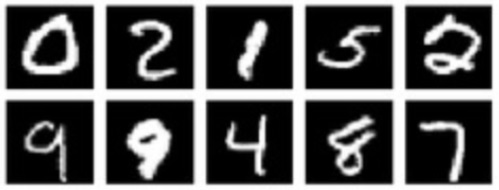
\includegraphics[scale=1]{mnist.png}
  	\caption{Ten pictures of handwritten digits from the MNIST dataset. \cite{MNIST}} \label{figMNIST}
\end{figure}

Two different models were trained on the MNIST dataset: A convolutional neural network consisting of 6 convolutional layers with 32 channels each with stride 1 and kernel size 5 followed by two fully connected layers with 1024 and 10 hidden units respectively. The second model is a feed-forward neural network with 6 fully connected layers of size 784 followed by a layer of size 10. Every convolutional and fully connected layer is preceded by batch normalization and followed by a ReLU layer. Both models use softmax as its last layer to convert the predictions into probablities that each image is one of $C=10$ classes where the classes correspond to the digits 0 to 9. The input to the convolutional neural network is a tensor of size $R \times 1 \times 28 \times 28$ and only uses one input channel since the images are in grayscale. For the feed-forward neural network the $28 \times 28$ images are reshaped into a 784-dimensional sized vector and stacked to form a tensor of size $R \times 784$. $R$ denotes the batch size.

Let $L(\theta)$ be the loss function used for the classification task. The cross entropy function is used which acts on two probability distributions: the predicted probabilities $\hat{y}$ and the real probabilities $\hat{y}$. Cross entropy and its partial derivative is defined by the following equations \cite{cs231n} \cite{notesonbackprop}: 
\begin{equation}\label{crossentropy}
L(\theta) = - \sum^{R }_{r=1} \sum^{C }_{c=1}y_{r,c} \ \log{\hat{y}_{r,c}}
\end{equation}
\begin{equation}\label{dydxcrossentropy}
\pd{L(\theta)}{\hat{y}_{r,c}} = - \frac{y_{r,c}}{\hat{y}_{r,c}}
\end{equation}

When training models, it is important to divide your data into a training set and a validation set. During training, the loss on the training set and the validation loss should be computed and tracked. However, only the loss of the training set should be used to train the neural network through Stochastic Gradient Descent. This is done to avoid overfitting the model on the training set. If the model is trained indefinitely on the training set it will learn to make extremely accurate predictions on exclusively the data it was trained on, failing to generalize to data it has not seen before. To combat this the loss or accuracy on the validation set is tracked and training is stopped when the validation accuracy stops improving.

For my own Python implementation of convolutional neural networks, the model was trained for 5 000 iterations on an a CPU with a learning rate of 0.001 and a batch size of 50. The total training time was 6 hours and the model achieved an accuracy of 99.2\% on the test set. Out of 10 000 handwritten the model had not seen previously it managed to classify 9 920 examples correctly. The implementation was deemed too computationally inefficient to do any further testing so I implemented the models in Facebook's GPU-accelerated tensor and dynamic neural network library PyTorch.

The models were trained for 100 000 iterations while tracking training and test loss simultaneously, as well as tracking the test accuracy, shown in figure \ref{figaccloss}. The initial learning rate was set to 0.001 and divided by 10 at 33 333 and 66 666 iterations. The models were trained on an Nvidia GTX 1080 ti for approximately 1 hour each. Note that the networks were only trained on the training set. Final results are shown in table \ref{tablemnist}.

\begin{figure}[h]
    \centering
    \subfloat[Accuracy]{{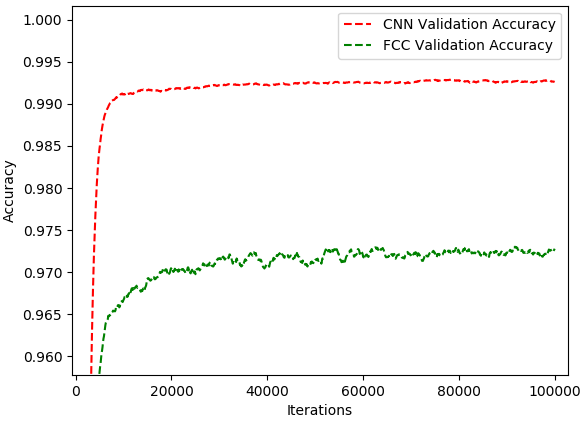
\includegraphics[width=8cm]{accuracy.png} }}
    \subfloat[Losses]{{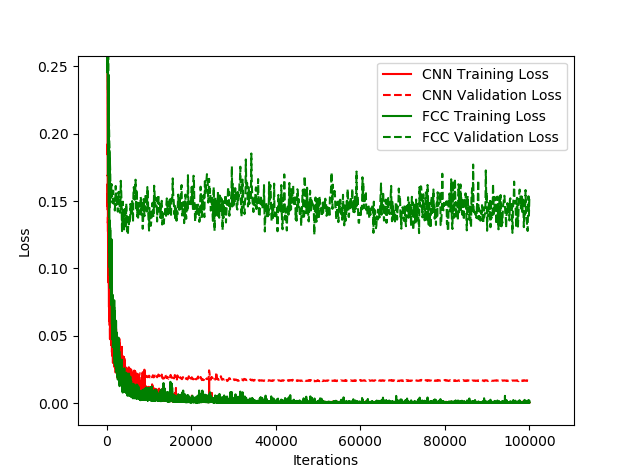
\includegraphics[width=8cm]{losses.png} }}
    \caption{The accuracy (a) and loss (b) of the convolutional model (CNN) and the feed-forward model (FCC) as a function of the numbers of iterations trained. The training loss is the loss on the training set and the validation loss is the loss on the test set. Accuracy is measured on the test set.} \label{figaccloss}
    
\end{figure}
\begin{table}[h]
\begin{center}
    \begin{tabular}{| l | l | l | l |}
    \hline
    Model & Accuracy & Validation loss \\ \hline
    Feed-forward Neural Network & 97.3\% & 0.15 \\ \hline
    Convolutional Neural Network & 99.5\% & 0.016 \\ \hline
    \end{tabular}
    \caption{The final accuracy and validation loss of the models. The accuracy is measured as the percentage of correctly classified examples from the test set of 10 000 never before seen images of handwritten digits. The validation loss is the loss on the test set.} \label{tablemnist}
\end{center}
\end{table}

The convolutional neural network is shown to have better generalizability on the test set than its feed-forward counterpart: While the training loss is the same for both the convolutional and feed-forward models, the validation loss is approximately 10 times higher for the feed-forward model. The final accuracy of the two networks were 99.5\% for the convolutional neural network and 97.3\% for the feed-forward neural network, tested on the test set consisting of 10 000 handwritten digits. 

\subsection{Dense face detection and localization}
For the task of detecting a variable number of faces in an iamge, the WIDERFace dataset \cite{WIDERFace} was used. It is a dataset consisting of 32 203 images of a total of 393 703 number of faces at different scales, lighting and occlusions. Every training example consists of a number of bounding boxes surrounding all the faces in the image. A bounding box consists of four coordinates specifying its location: two for the upper left corner and two for the bottom right corner of the bounding box. The images are labaled by humans and is called the ground truth of the image. 

A convolutional neural network can be used to detect up to thousands of different faces in a single picture or video in real time. A custom region based one-shot detector is used to achieve this. One-shot detectors were first introduced in the paper \textit{You Only Look Once: Unified, Real-Time Object Detection} \cite{yolo} and later modified and improved in the papers \textit{SSD: Single Shot MultiBox Detector} \cite{ssd}, \textit{YOLO9000: Better, Faster, Stronger} \cite{yolo9000}, \textit{DSSD: Deconvolutional Single Shot Detector}  \cite{dssd} and \textit{Focal Loss for Dense Object Detection} \cite{retinanet}. A one-shot detector works by predicting up to tens of thousands of bounding boxes in different spatial positions in an image, that sets out to detect every object in that image. In addition to predicting the bounding box coordinates, the model predicts probability scores of how likely it is that there exists an object inside of the bounding box.   

I constructed a model termed FaceResNet based on the current state of the art in object detection: RetinaNet \cite{retinanet}. It uses a feature pyramid architecture, introduced in the paper \textit{"Feature Pyramid Networks for Object Detection"} \cite{fpn}, to be able to use feature maps from different depths in the neural network to predict objects of different scales. The backbone network RetinaNet uses for the feature pyramid network is a ResNet-101 \cite{resnet}. The model predicts the bounding boxes by basing their predictions on a number of anchor boxes at different scales and positions in the image. For every anchor box, the network predicts four coordinate offsets to shift the anchor box with and a set of probabilities of there existing an object inside the predicted bounding box. This process is applied to every pyramid level. RetinaNet uses pyramid layers P3 throughout P7 and uses anchor boxes of sizes $32^2$ to $512^2$. Let the pyramid layers width and height be $W$ and $H$ and let $A$ denote the number of differently shaped anchor boxes at every pyramid layer. In total the pyramid layers will have $WHA$ unique anchor boxes spaced out evenly throughout every pyramid level. The coordinate offset regression and class probability classification for every anchor box are done by two smaller subnetworks called the regression head and the classification head (see figure \ref{figretinanet}). The classification head predicts $KWHA$ probabilities where $K$ is the number of object classes. $K$ consists of $1$ foreground class (no object in the bounding box) and $K-1$ foreground classes (objects). The regression head predicts $4WHA$ coordinate offsets: four offsets for every bounding box.  

\begin{figure}[h]
	\centering
  		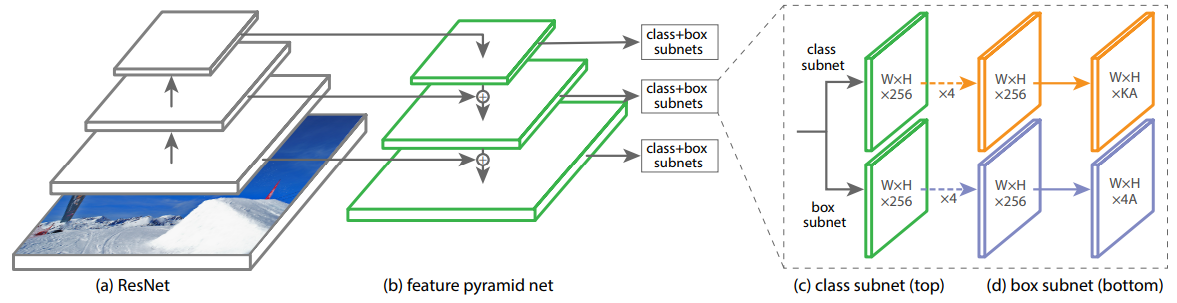
\includegraphics[scale=0.38]{retinanet.png}
  	\caption{The architecuture of RetinaNet. The last feature maps of every pyramid level is fed into a classification and regression head. \cite{retinanet}}\label{figretinanet}
\end{figure}

My model FaceResNet differs from RetineNet by using a ResNet-50 as a backbone network and by using $A=6$ anchor boxes at every pyramid level of sizes $16^2$ to $416^2$ pixels, scaled by a factor of $2^\frac{1}{3}$, and using 2 different aspect ratios: 1:1 and 1:1.5 (width:height). Additionally, both subnetworks use a completely different architecture: Instead of using 5 normal $3 \times 3$ convolutions, FaceResNet uses 8 residual bottleneck building blocks; the same building blocks used in the ResNet architecture. FaceResNet only predicts $K=2$ class probabilities: if the bounding box contains a face or not.

The model is trained by assigning every anchor box either a negative or a positive label, depending on if the anchor box contains a ground truth object. An anchor box is said to contain an object if the intersection over union (IoU) \cite{iou} of the area of the anchor box and the area of the ground truth is bigger or equal to 0.5. The intersection over union is used to determine how similar two sets $A$ and $B$ are (see figure \ref{figiou}). It is defined by the following equation: 

\begin{equation}\label{eqiou}
IoU(A, B)=\frac{|A \cap B|}{|A \cup B|}
\end{equation}

\begin{figure}[h]
	\centering
  		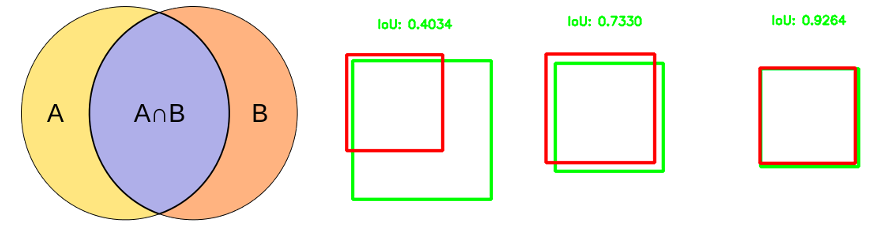
\includegraphics[scale=0.5]{iou.png}
  	\caption{IoU \cite{iou} is defined as the size of the union divided by the size of the intersection of two sets $A$ and $B$. A bigger IoU implies that the predicted bounding box is closer to the ground truth. } \label{figiou}
\end{figure}

The loss function $L(\theta)$ used by FaceResNet is a combination of a coordinate regression loss $L_r$, and a bounding box classification loss $L_c$. $L_r$ is the Smooth L1 Loss \cite{cs231n} defined by equation \eqref{eqsmoothl1loss}. $L_c$ is the Focal Loss \cite{retinanet} defined by equation \eqref{eqfocalloss}. The hyperparameters used by FaceResNet for the Focal Loss are the same as for RetinaNet, namely, $\gamma=2$ and $\alpha = 3$ for the foreground class.

\begin{equation}\label{eqfocalloss}
L_r(x) = \begin{cases}
				0.5x^2 & \mbox{om } |x| < 1\\
				|x| - 0.5 & \mbox{otherwise}\\
			\end{cases}
\end{equation}

\begin{equation}\label{eqsmoothl1loss}
L_c(p, \hat{p}) = - \alpha (1-p)^{\gamma}p \log{\hat{p}}
\end{equation}

The total loss $L(\theta)$ used by FaceResNet is the mean of the regression losses $L_r$ for all positively assigned anchors plus the mean of the classification losses for all anchor boxes. Negatively assigned anchors do not have any effect on the regression loss. Let $r_a$ and $\hat{r}_a$ be the predicted and ground truth coordinate offsets for anchor box $a$. Let $p_a$ and $\hat{p}_a$ be the predicted and ground truth probability score for anchor $a$ to contain an object. $N$ is the number of anchor boxes and $N_{pos}$ is the number of positively assigned anchor boxes. The total loss can then be described by the following equation:
\begin{equation}
\begin{split}
	L(\theta) = &  \frac{1}{N} \sum_{a \in anchors} L_c(p_a, \hat{p}_a) \\
	& + \frac{1}{N_{pos}} \sum_{a \in positive} L_r(r_a - \hat{r}_a)  \\ 
\end{split}
\end{equation}

The model was trained for 700 000 iterations on an Nvidia GTX 1080ti with an initial learning rate of 0.001. Due to memory limitations a batch size of 2 had to be used, the bare minimum for batch normalization to function. Every input image was randomly resized to be of size $512^2$ or $640^2$. Following industry standards for data augmentation, the network was trained on random image crops of the training data to artificially increase the size of the dataset. Additionally, the image was flipped horizontally with a probability of 0.5 and random color jitter was applied. Figures \ref{resultscrowd3} - \ref{resultscrowd} show quantitative results on images not found in the WIDERFace data set.

\begin{figure}[h] %0.185   0.11
\begin{center}
  		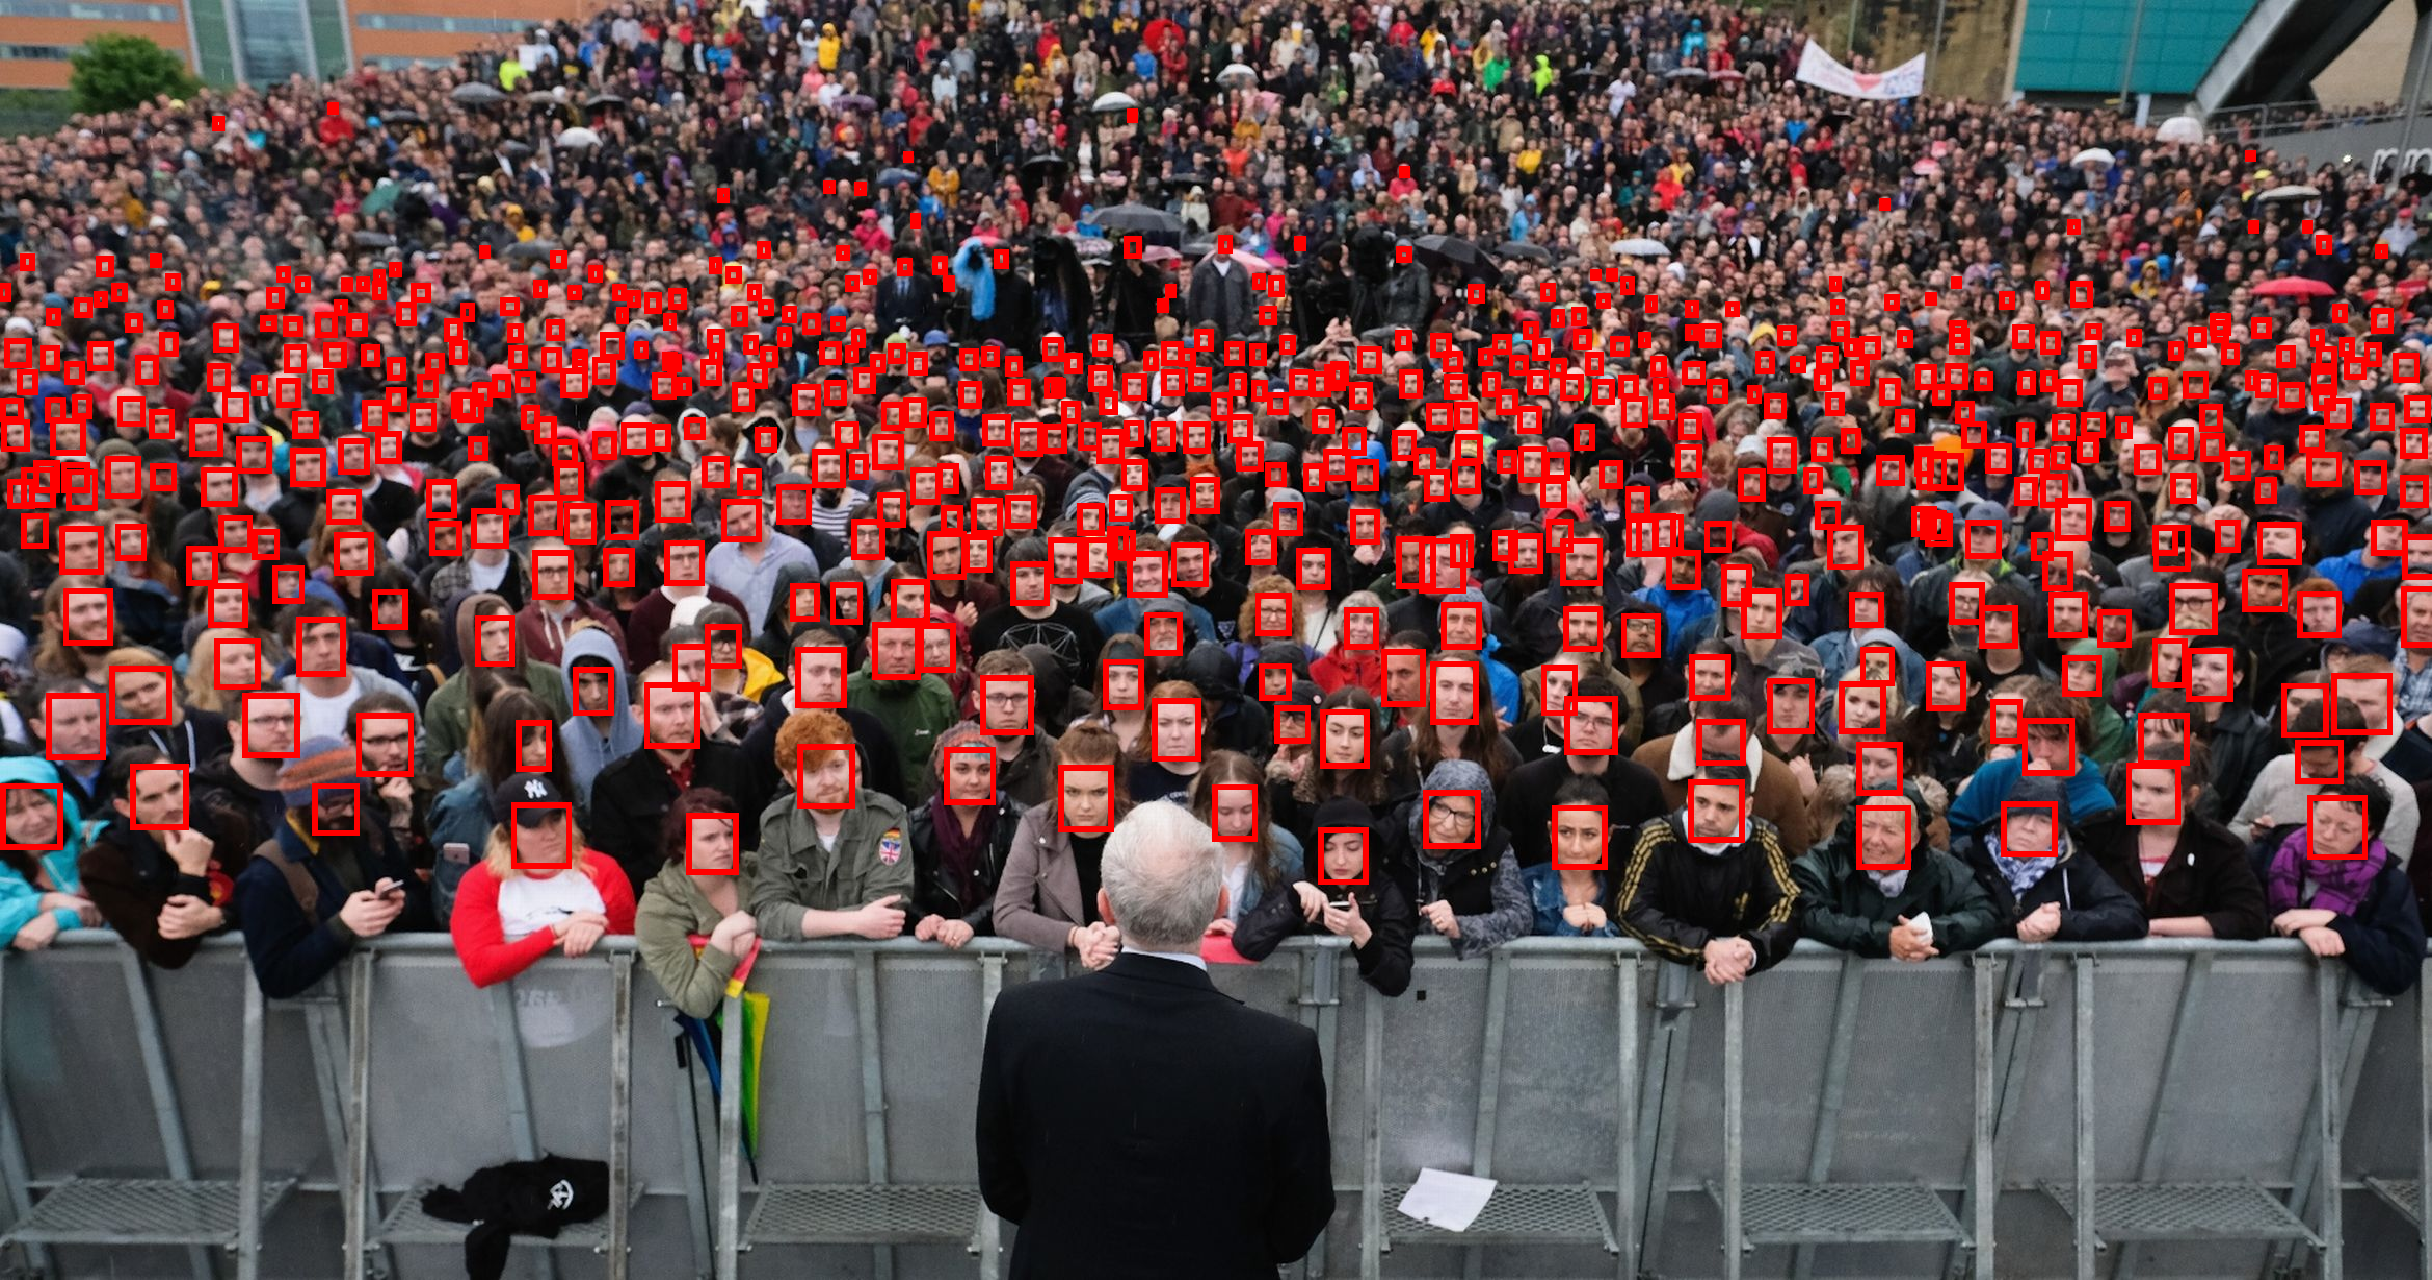
\includegraphics[scale=0.17]{resultscrowd3.png}
  		\caption{Qualitative results of the model FaceResNet.}\label{resultscrowd3}
\end{center}
\end{figure}
\begin{figure}[h]
\begin{center}
  		\includegraphics[scale=0.101]{resultscrowd4.png}
  		\caption{Qualitative results of the model FaceResNet.}\label{resultscrowd4}
\end{center}
\end{figure}
\begin{figure}[h]
\begin{center}
  		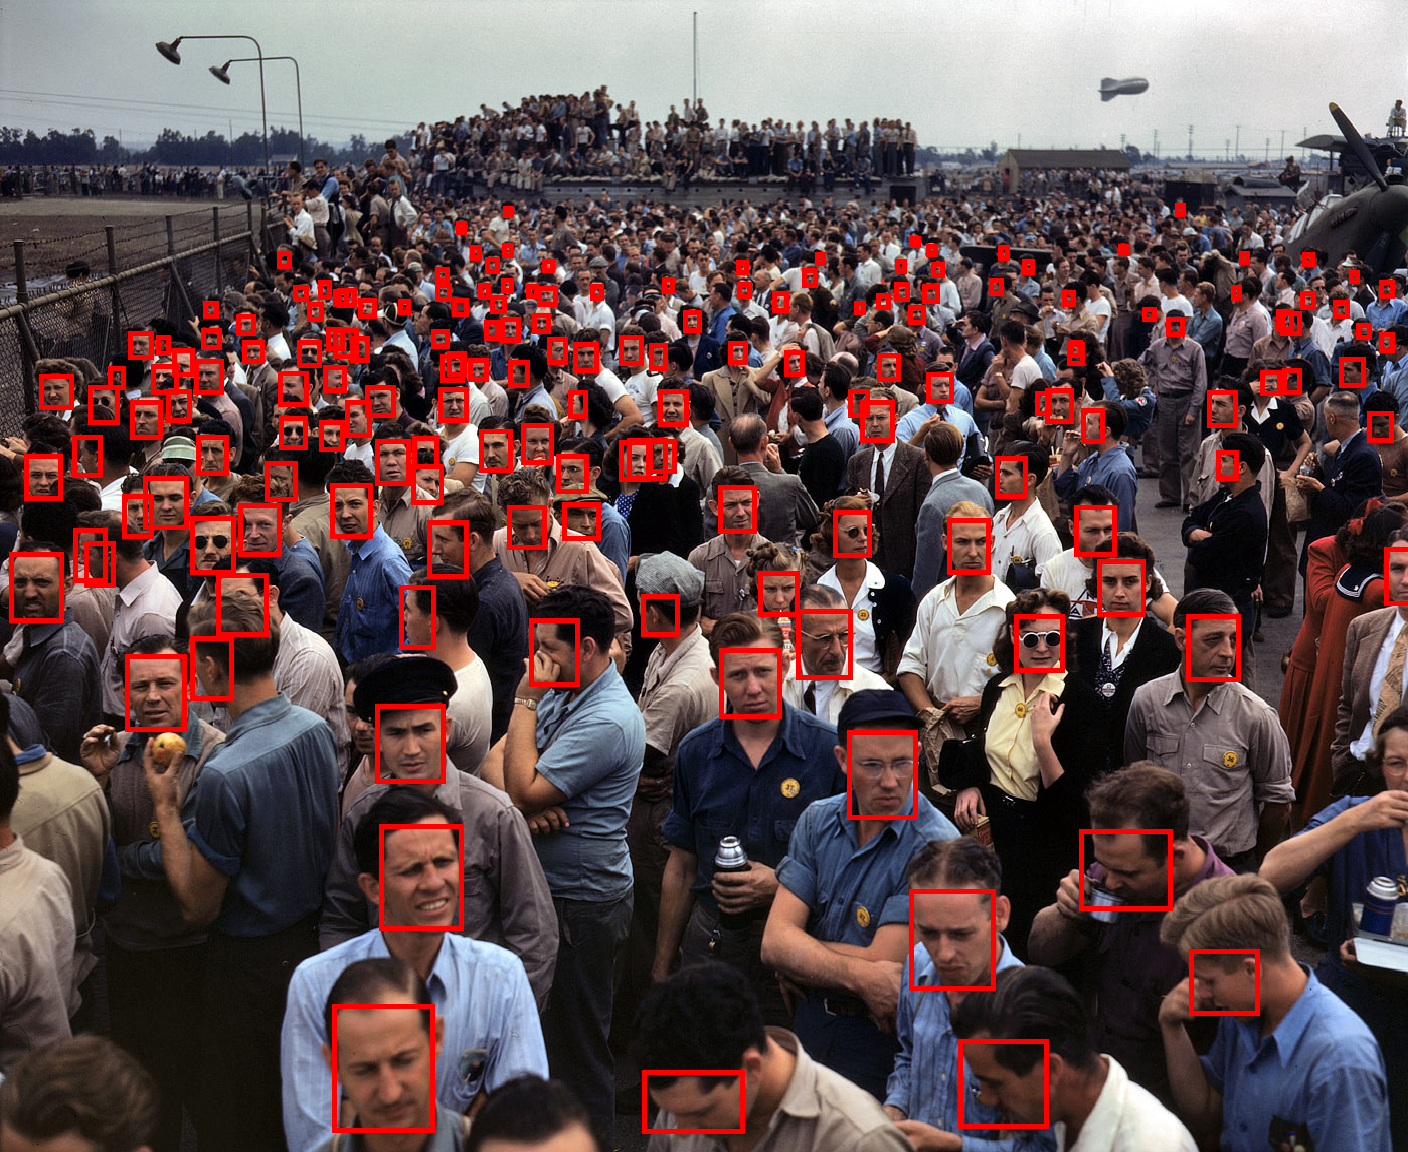
\includegraphics[scale=0.32]{resultscrowd.png}
  		\caption{Qualitative results of the model FaceResNet.}\label{resultscrowd}
\end{center}
\end{figure}

One forward pass of an image of size $512^2$ takes 30 ms, enabling the model to be used in real time for real time applications. The model can for instance be applied to CCTV applications for security cameras or be used as a face detector for automatic tagging on social media or face detection in digital cameras.

An area where FaceResNet shows weakness is in detecting small faces. This can be due to there not being enough information in the image for the model to accurately detect the small faces since they only consist of $16$ pixels in width and height. Another reason could be that the classification error of the negative boxes dominates the error of the positive boxes. Since the small bounding boxes are created from the lowest pyramid layer with the biggest spatial height and with, more smaller than bigger bounding boxes are created, while the number of ground truth boxes stays constant for approximately all sizes. The ratio of negative to positive bounding boxes is bigger for the small anchors, resulting in detection performance for small faces.

\section{Conclusion} 
Feed-forward and convolutional neural networks are a type of artificial neural network consisting of sequential layers of neurons. In a feed-forward neural network every neuron from the previous layer is connected to all the neurons in the proceeding layer. In a convolutional neural network, only nearby neurons are connected to the neurons of the proceeding layer through what is called the convolution operation. Forward propagation is the the process of forwarding the signal from your input neurons to your output neurons through the neural network. Backpropagation is the method of training the neural network through repeated use of the chain rule to find how the neural network's parameters should be modified to minimize a determined loss function. Classification of handwritten
digits was achieved by using a 7 layer deep feed-forward neural network with hidden layer sizes 1000, as well by using a 7 layer deep convolutional neural network with kernel size 5, followed by two fully connected layers. Additionally, a deep convolutional neural network based on a state of the art one-shot detector was used to detect a variable number of faces in an image.

\begin{thebibliography}{99}	
 \bibitem{cs231n} 
	\textit{CS231n: Convolutional Neural Networks for Visual Recognition.}
    F. Li, A. Karpathy and J. Johnson.
	Stanford University, university course, winter 2016.
	
	\bibitem{batchnorm} 
	\textit{Batch normalization: Accelerating deep network training by reducing internal covariate shift.}
    S. Ioffe and C. Szegedy. 
	arXiv preprint arXiv:1502.03167, 2015.

\bibitem{eigen}
\textit{Eigen v3}.
G. Guennebaud and B. Jacob and others. URL http://eigen.tuxfamily.org. 2010

\bibitem{numpy}
\textit{The NumPy Array: A Structure for Efficient Numerical Computation, Computing in Science \& Engineering, 13, 22-30}.
S. van der Walt, S. C. Colbert and G. Varoquaux.  (2011), DOI:10.1109/MCSE.2011.37 

 

\bibitem{tensorflow}
\textit{TensorFlow: Large-scale machine learning on heterogeneous systems},
M. Abadi, A. Agarwal, P. Barham, E. Brevdo,
Z. Chen, C. Citro, G. Corrado, A. Davis,
J. Dean, M. Devin, S. Ghemawat, I. Goodfellow,
A.Harp, G. Irving, M. Isard, R. Jozefowicz, Y. Jia,
L. Kaiser, M. Kudlur, J. Levenberg, D. Mané, M. Schuster,
R. Monga, S. Moore, D. Murray, C. Olah, J. Shlens,
B. Steiner, I. Sutskever, K. Talwar, P. Tucker,
V. Vanhoucke, V. Vasudevan, F. Viégas,
O. Vinyals, P. Warden, M. Wattenberg, M. Wicke,
Y. Yu, and X. Zheng.
URL https://www.tensorflow.org/.
2015.

\bibitem{pytorch}
\textit{Automatic differentiation in PyTorch}.
A. Paszke,   S. Gross, S. Chintala,   G. Chanan,   E. Yang,   Z. DeVito,   Z. Lin,   A. Desmaison,   L. Antiga,  and A. Lerer
2017

\bibitem{hidden12}
	\textit{A simple neural network with Python and Keras}.
	A. Rosebrock.
	PyImageSearch
	URL https://www.pyimagesearch.com/.
	26 September 2016.
	
\bibitem{wikiStanford} 
	\textit{Unsupervised Feature Learning and Deep Learning.}
    Standford University, Department of Computer Science.
    URL http://ufldl.stanford.edu/wiki/.
	Last updated 31 Mars 2013.	
	

	
\bibitem{gradient} 
	\textit{Scientific Computing 2013, Worksheet 6: Optimization: Gradient and steepest descent.}
    University of Tartu, Estonia.
    2013.
    
\bibitem{convmath} 
	\textit{Introduction to Convolutional Neural Networks.}
    J. Wu. 
    National Key Lab for Novel Software Technology, Nanjing University, China.
    1 May, 2017.
    
\bibitem{figSGD}
	\textit{Tuning the learning rate in Gradient Descent.}
	 V. Vryniotis.
	URL http://blog.datumbox.com/tuning-the-learning-rate-in-gradient-descent/.
	27 October 2013.    
   
\bibitem{convarithmetic} 
	\textit{A guide to convolution arithmetic for deep learning.}
    V. Dumoulin  and F. Visin.
    FMILA, Université de Montréal. AIRLab, Politecnico di Milano.
	24 mars, 2016.
	
\bibitem{vgg}
	\textit{Very Deep Convolutional Networks for Large-Scale Image Recognition.}
	K. Simonyan and
    A. Zisserman.
    arXiv preprint arXiv:1409.1556, 2014
    
    



	
\bibitem{figkonv}
	\textit{Understanding Convolutional Neural Networks for NLP.}
	D. Britz.
	WildML, Artificial Intelligence, Deep Learning, and NLP.
	7 November 2015.
	
	
	
\bibitem{figconv}
	\textit{Deep learning for complete beginners: convolutional neural networks with keras.}
	P. Veličković.
	Camebridge Spark. 
	URL https://cambridgespark.com/content.
	Last updated 20 Mars 2017.
	
	    
\bibitem{webconv1} 
	\textit{Backpropagation In Convolutional Neural Networks.}
	J. Kafunah.
    DeepGrid, Organic Deep Learning. 
    URL http://www.jefkine.com/.
	5 September 2016.
	
	
\bibitem{webconv2} 
	\textit{Note on the implementation of a convolutional neural networks.}
	C. Thorey.
    Machine Learning Blog. 
    URL http://cthorey.github.io/.
	2 February 2016.
	
	
	
\bibitem{webconv3} 
	\textit{Convolutional Neural Networks.}
	A. Gibiansky.
    URL http://andrew.gibiansky.com.
	24 February 2014.
	
	
	

	
\bibitem{webBN1} 
	\textit{What does the gradient flowing through batch normalization looks like?}
	C. Thorey.
    Machine Learning Blog. 
    URL http://cthorey.github.io/.
	28 January 2016.
	
	

	
\bibitem{webBN2} 
	\textit{Understanding the backward pass through Batch Normalization Layer.}
	Flaire of Machine Learning
    URL https://kratzert.github.io.
	5 September 2016.

\bibitem{notesonbackprop} 
	\textit{Notes on Backpropagation.}
    P. Sadowski.
    University of California Irvine	Department of Computer Science.
    


	
\bibitem{websoftmax} 
	\textit{Classification and Loss Evaluation - Softmax and Cross Entropy Loss.}
	P. Dahal. 
	DeepNotes.
    URL https://deepnotes.io/softmax-crossentropy.
	24 February 2014.
	
\bibitem{MNIST}
	\textit{The MNIST database of handwritten digits}
	Y. LeCun, C. Cortes and C. Burges. Courant Institute, NYU. Google Labs, New York. Microsoft Research, Redmond. 
	URL http://yann.lecun.com/exdb/mnist/.
	3 November 2017.
	
	
	
    
\bibitem{WIDERFace}
	\textit{WIDER FACE: A Face Detection Benchmark.}
	Yang, Shuo and Luo, Ping and Loy, Chen Change and Tang, Xiaoou
    IEEE Conference on Computer Vision and Pattern Recognition (CVPR), 2016
    
    
    
    

    
\bibitem{yolo} 
	\textit{You only look once: Unified, real-time object detection.}
    J. Redmon, S. Divvala, R. Girshick, and A. Farhadi. 
    arXiv preprint arXiv:1506.02640, 2015.
    
    
    
\bibitem{ssd}
	\textit{{SSD:} Single Shot MultiBox Detector.}
	W. Liu and
               D. Anguelov and
               D. Erhan and
               C. Szegedy and
               S. Reed and
               C. Fu and
               A. Berg.
    arXiv preprint arXiv:1512.02325, 2015


    
\bibitem{yolo9000} 
	\textit{{YOLO9000:} Better, Faster, Stronger.}
    J. Redmon and
               A. Farhadi. 
    arXiv preprint arXiv:1612.08242, 2016.
    
    
    
    
    
\bibitem{dssd}
	\textit{{DSSD} : Deconvolutional Single Shot Detector.}
	C. Fu and
               W. Liu and
               A. Ranga and
               A. Tyagi and
               A. C. Berg
    arXiv preprint arXiv:1701.06659, 2017
    
    
    
\bibitem{retinanet}
	\textit{Focal Loss for Dense Object Detection.}
	Tsung{-}Yi Lin,
    Priya Goyal,
    Ross B. Girshick,
    Kaiming He and
    Piotr Doll{\'{a}}r.
    arXiv preprint arXiv:1708.02002, 2017

\bibitem{fpn}
	\textit{Feature Pyramid Networks for Object Detection.}
	Tsung{-}Yi Lin,
               Piotr Doll{\'{a}}r,
               Ross B. Girshick,
               Kaiming He,
               Bharath Hariharan and
               Serge J. Belongie.
    arXiv preprint arXiv:1612.03144, 2016
    

\bibitem{resnet} 
	\textit{Deep residual learning for image recognition.}
    K. He, X. Zhang, S. Ren, and J. Sun. 
    arXiv preprint arXiv:1512.03385, 2015.

    
\bibitem{iou}
	Jaccard Index. Wikipedia.
    URL https://en.wikipedia.org/wiki/Jaccard{\_}index. 
    20 January 2018


%-----------------------------------
%-----------------------------------
%-----------------------------------
%-----------------------------------
%-----------------------------------


\end{thebibliography}


\end{document}